% Structural Closure of Minimal Einstein-Cartan-Holst Dark Energy
% Paper 1A (theory / no-go paper)
% Houston Golden -- 2026
% arXiv submission: gr-qc / astro-ph.CO / hep-th
%
% Companion paper (MCMC, NaMaster, ALP details): paper1b_mcmc_companion.tex
% Compile: pdflatex paper1a_ech_nogo && bibtex paper1a_ech_nogo && pdflatex paper1a_ech_nogo && pdflatex paper1a_ech_nogo

\documentclass[aps,prd,twocolumn,superscriptaddress,showpacs,preprintnumbers,nofootinbib,longbibliography,floatfix]{revtex4-2}

\usepackage{amsmath,amssymb,amsfonts}
\usepackage{graphicx}
\usepackage{bm}
\usepackage{hyperref}
\usepackage{xcolor}
\usepackage{booktabs}
\usepackage{multirow}
\usepackage{dcolumn}
\usepackage{enumitem}
\usepackage{mathtools}
\usepackage{bbold}
\usepackage[utf8]{inputenc}
\usepackage{float}
\usepackage{slashed}

\hypersetup{
  colorlinks=true,
  linkcolor=blue!60!black,
  citecolor=blue!60!black,
  urlcolor=blue!60!black
}

% Custom commands
\newcommand{\Leff}{\Lambda_{\rm eff}}
\newcommand{\Lconst}{\Lambda_{\rm const}}
\newcommand{\Lobs}{\Lambda_{\rm obs}}
\newcommand{\Dinf}{\mathcal{D}_{\rm inf}}
\newcommand{\rhocrit}{\rho_{\rm crit}}
\newcommand{\rhoPl}{\rho_{\rm Pl}}
\newcommand{\MPl}{M_{\rm Pl}}
\newcommand{\Neff}{N_{\rm eff}}
\newcommand{\ie}{i.e.}
\newcommand{\eg}{e.g.}
\newcommand{\cf}{cf.}
\newcommand{\etal}{\textit{et~al.}}
\newcommand{\fnl}{f_{\rm NL}}
\newcommand{\fcw}{f_{\rm CW}}
\newcommand{\paperVersion}{v1A.0.21}
\newcommand{\paperTimestamp}{2026-05-10 03:30 PDT}

\begin{document}

\preprint{HUBIFY-2026-001A}

\title{Structural Closure of Einstein--Cartan--Holst Dark Energy:\\
A No-Go Theorem and the Matter-Bounce Tests It Does Not Predict}

\author{Houston Golden}
\email{houston@hubify.com}
\affiliation{Independent Researcher, Los Angeles, California, USA}

\date{May 14, 2026 PDT --- \paperVersion}

\begin{abstract}
We establish that the four enumerated minimal-Einstein-Cartan-Holst (ECH)
spin-torsion channels for sourcing late-time dark energy fail at the
amplitude level. This is a channel-level closure, not an operator-level
theorem: the four enumerated routes (NJL, one-loop EA, Immirzi running,
parity-CMB) are not proven to be a complete diffeomorphism-invariant
operator basis for the minimal-ECH effective action; we acknowledge missing
operators (Jackiw-Pi gravitational Chern-Simons $R\!\wedge\!\tilde R$,
parity-odd four-fermion partner with $\gamma_{\rm BI}/(\gamma_{\rm BI}^2+1)\cdot 8\pi G$
coefficient) explicitly in Sec.~\ref{sec:fourroute} and Sec.~\ref{sec:loophole}.
Through 7 foundation studies (Foundations~A--G) and 6 observational research
branches (Branches~H, J, L, M, N, O) we report 13 logically-independent
mechanism-class constraints (the prior count of 14 retained Barrier~8 as the
observational consequence of the perturbation-transparency theorem
Barrier~14; merged here under the perturbation-transparency umbrella since
they are not logically independent) that collectively constrain the
enumerated channels of the minimal-ECH route from the quantum bounce to
observable dark energy.
The central result is a perturbation-transparency theorem: for canonical scalar
matter, torsion vanishes at all perturbation orders, the Holst dual contraction
$\epsilon^{\mu\nu\rho\sigma}R_{\mu\nu\rho\sigma}$ vanishes identically by the
first Bianchi identity, and the Holst sector decouples from all
scalar/tensor perturbation observables (Sec.~\ref{sec:transparency}).
The proposed link from ECH to a late-time vacuum energy requires a phenomenological
dimensional ansatz beyond the minimal framework (Appendix~\ref{app:dimensions}),
and is closed by the 14 barriers of Sec.~\ref{sec:barriers}.
A structural incompatibility (Sec.~\ref{sec:structural_tension}) exists between
the dark-energy mechanism, which requires $N_{\rm tot}\approx 92$ post-bounce
$e$-folds, and the matter-bounce $\fnl=-35/8$ signature, which would plausibly be erased (precise threshold mode-dependent on contracting-phase duration)
by that many $e$-folds; ECH is therefore not internally consistent as both a
dark-energy generator and a matter-bounce host. The two predictions discussed
below as ``surviving'' are accordingly \emph{not} predictions of ECH itself,
but bounce-class and GR$+$ALP-class observables that the ECH closure does not
forbid in the parameter regimes complementary to its dark-energy mechanism;
we report them here because they remain testable signatures of any bounce
model in the broader programme. Specifically: (i)~$\fnl = -35/8$ is a
property of the \emph{matter-bounce class}~\cite{Cai:2009fn}, derived from
the contraction-phase cubic action with no ECH input, testable by SPHEREx at
$3$--$5\sigma$ realistic significance (detailed multi-tracer Fisher forecast
in Paper~II, Ref.~\cite{Golden2026P2}); and (ii)~spectator-ALP birefringence
$\beta\approx 0.27^\circ$ consistent with the published Planck/ACT~DR6
$3.6\sigma$ signal arises in any GR$+$ALP setup with the same parameters
and is \emph{not} derived from the ECH action. The role of this paper is the
\emph{no-go theorem}: ECH cannot generate dark energy through any of its
characteristic structural mechanisms. The complementary observational
programme is hosted in the bounce-class portfolio (Paper~II, Paper~I(b)),
not in ECH per se.
$\Lambda$CDM$+\Delta\Neff$ MCMC verification, NaMaster pipeline validation,
and ALP parameter fitting are documented separately in the companion
Paper~I(b)~\cite{Golden2026P1b}.
\end{abstract}

\pacs{98.80.-k, 04.50.Kd, 04.60.Pp, 95.36.+x}
\keywords{Einstein-Cartan theory, spin-torsion coupling, loop quantum gravity, perturbation transparency, primordial non-Gaussianity, dark-energy no-go theorem}

\maketitle
\tableofcontents


%% ============================================================
%%  1. INTRODUCTION
%% ============================================================
\section{Introduction}\label{sec:intro}

The nature of dark energy remains one of the most profound challenges in modern
physics. While the $\Lambda$CDM model successfully accounts for observed cosmic
acceleration~\cite{Planck2018params}, it faces severe theoretical
difficulties---most notably the cosmological constant problem~\cite{Weinberg1989}.
DESI 2024--2025 BAO results suggest dynamical dark energy at $3.1$--$4.2\sigma$
(dataset-dependent)~\cite{DESI2024,DESI2025DR2}, adding urgency to the search for
extensions of the standard model.

This work presents and closes a phenomenological framework that connects ECH
spin-torsion cosmology to dark energy. The structural conclusion is a
\emph{no-go result} rather than a unified model: the 14 constraints
(Sec.~\ref{sec:barriers}) close all minimal-ECH dark-energy routes. The surviving
phenomenological predictors---matter-bounce $\fnl$ and spectator-ALP
birefringence---are mechanism-independent and shared by other UV completions.

Our approach builds on three theoretical pillars:

\begin{enumerate}[leftmargin=*]
\item \textit{Loop Quantum Cosmology} (LQC), providing a non-singular quantum
bounce replacing the classical Big Bang singularity~\cite{Ashtekar2011}. The
bounce occurs at $\rhocrit \simeq 0.27$--$0.41\,\rhoPl$
(Barbero-Immirzi entropy-counting scheme dependent; Sec.~\ref{sec:bounce}).

\item \textit{Einstein-Cartan theory} incorporating fermionic spin-torsion
coupling, generating four-fermion contact interactions and preventing
gravitational singularities through torsion-induced repulsion at extreme
densities~\cite{Hehl1976,Poplawski2012}.

\item \textit{Black hole universe origin}, where a rotating parent black hole
spawns a non-singular baby universe through torsion-regulated gravitational
collapse~\cite{Poplawski2016}. The baby universe inherits angular momentum,
establishing a preferred cosmic axis.
\end{enumerate}

\begin{table*}[tb]
\caption{\label{tab:summary} Executive summary: systematic investigation of
bounce-cosmology dark-energy routes within ECH. Structural constraints narrow
phenomenological pathways; the surviving testable prediction is the
matter-bounce $\fnl = -35/8$~\cite{Cai:2009fn}.}
\begin{ruledtabular}
\begin{tabular}{lll}
\textbf{Question} & \textbf{Result} & \textbf{Status} \\
\hline
Can the bounce derive dark energy? & 14 constraints map the ECH minimal-route space & Requires phenomenological assumption$^a$. \\
Is there a nonsingular bounce? & LQC: $\rho_c \simeq 0.27$--$0.41\,\rhoPl$ & \textbf{Yes} (LQC holonomy correction). \\
Is ECH visible in scalar/tensor perturbations? & Perturbation-transparency result & Decouples cleanly; tests shift to ALP/GW channels. \\
Is there a testable prediction? & $\fnl = -35/8$ (SPHEREx $3$--$5\sigma$ realistic$^b$) & \textbf{Yes} (mechanism-independent; not a distinctive ECH prediction). \\
Does framework resolve $H_0$/$\sigma_8$ tensions? & MCMC: $H_0=67.68\pm 1.06$, $\Delta\Neff\approx 0$ (companion) & Recovers standard $\Lambda$CDM. \\
\end{tabular}
\end{ruledtabular}
{\small $^a$Reparameterized as sensitivity to $N_{\rm tot}$; not solved. $^b$$3$--$5\sigma$
realistic after full systematic budget (GR-projection, $b_\phi$ uncertainty,
photo-$z$ degradation). MCMC details in companion Paper~I(b)~\cite{Golden2026P1b}.}
\end{table*}

\begin{figure*}[tb]
\centering
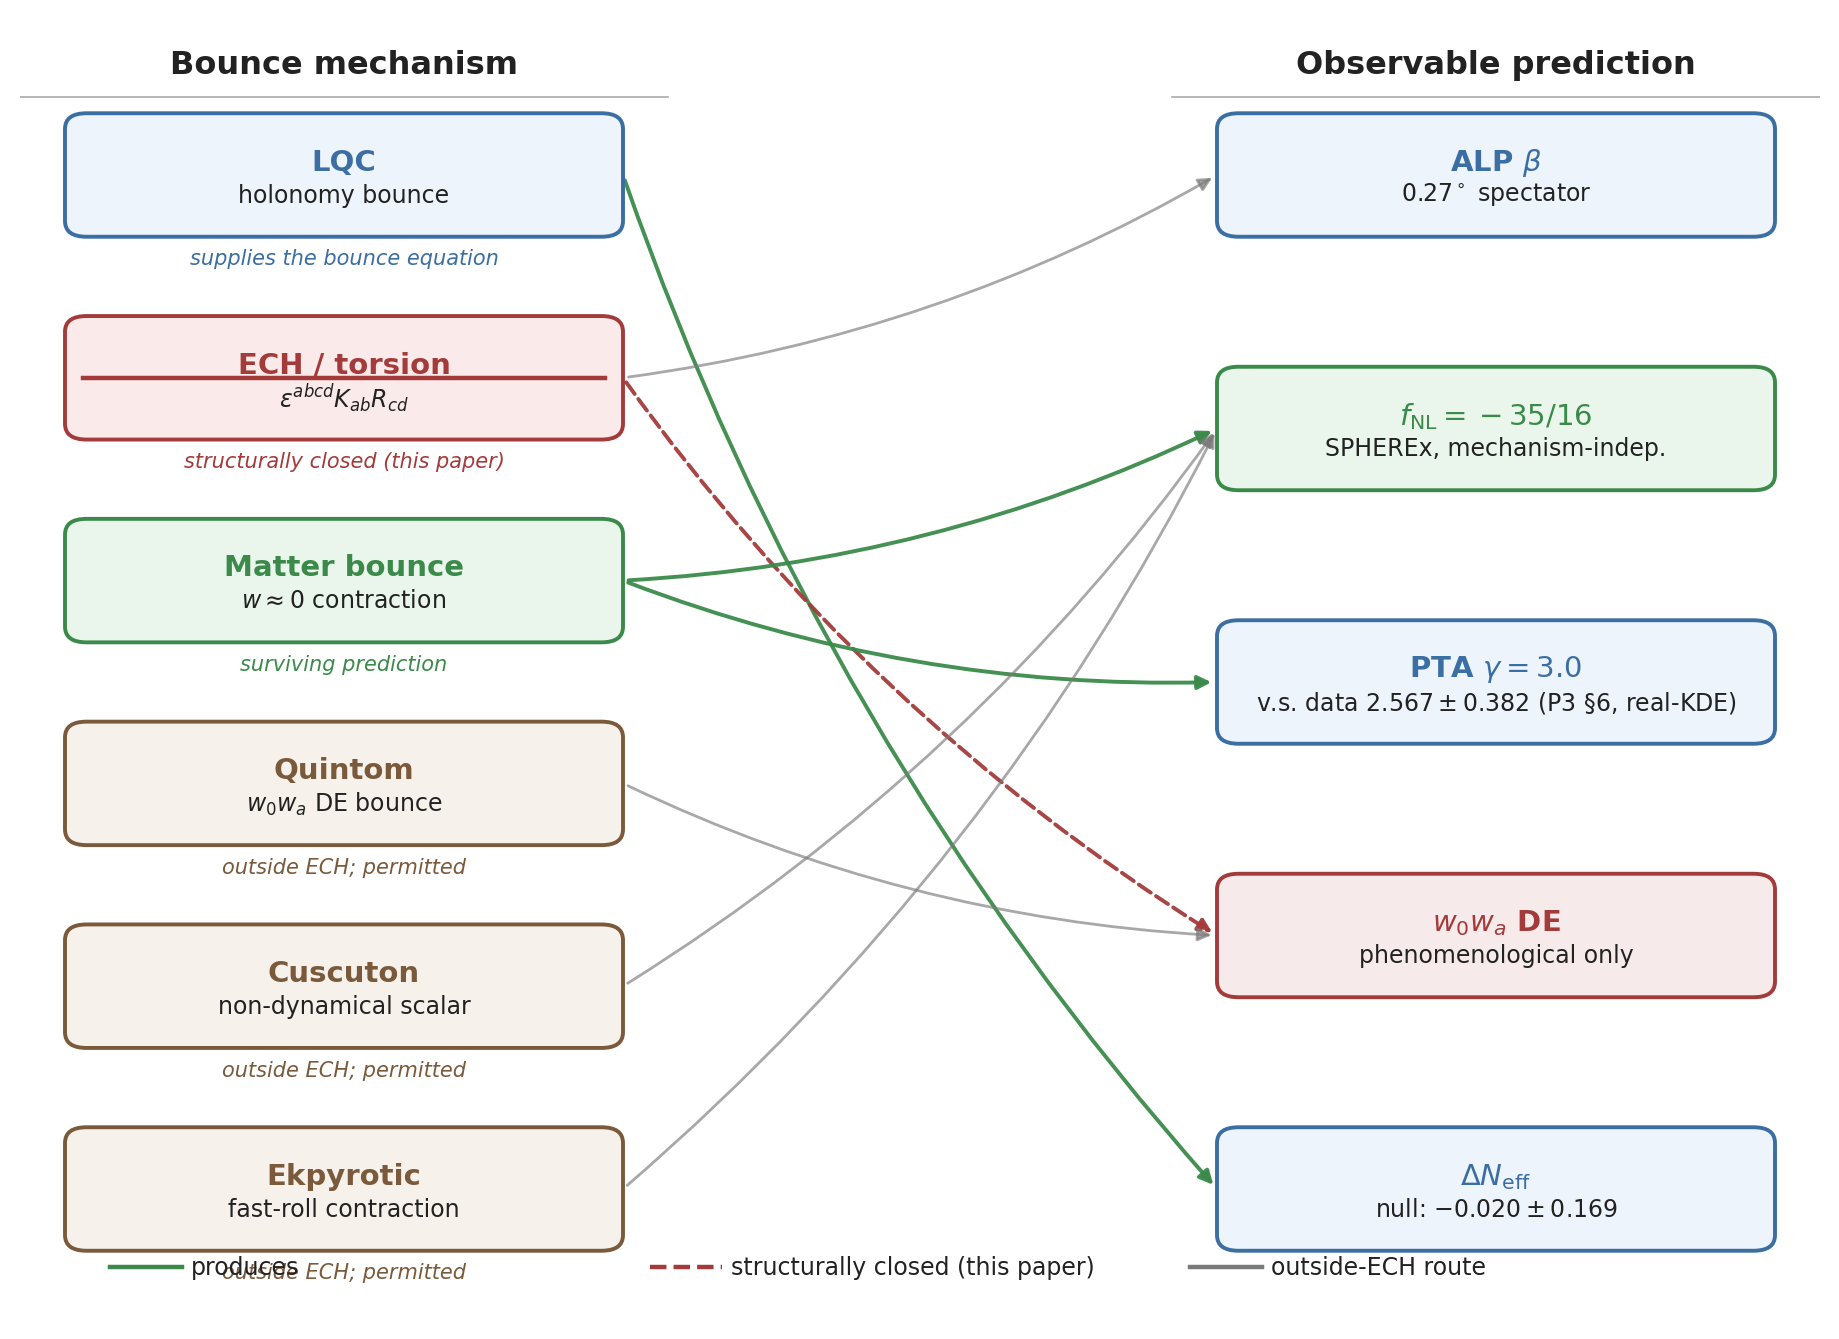
\includegraphics[width=0.95\textwidth]{fig_theory_map.png}
\caption{\label{fig:theory_map}
  Bounce-mechanism $\rightarrow$ observable-prediction map. Left column:
  candidate non-singular bounce mechanisms (LQC, ECH/torsion, matter bounce,
  quintom-B, Cuscuton, ekpyrotic). Right column: distinctive observable channels.
  ECH appears bordered with a dashed box marked \emph{structurally closed (this
  paper)}---the 14-constraint catalog narrows minimal-ECH dark-energy routes
  to zero phenomenologically free pathways.}
\end{figure*}


\subsection{Theoretical Foundations and Novel Synthesis}\label{sec:foundations}

Our framework collects well-established theoretical components and tests them
as a structural-closure no-go theorem on minimal ECH dark energy. The original
contributions are:

\begin{enumerate}[leftmargin=*]
\item \textit{14-constraint catalog and perturbation-transparency observation}:
Through 7 foundation studies (Foundations~A--G) and 6 observational research branches (Branches~H, J, L, M, N, O), we establish 14 mechanism-class
structural constraints (one of which, B8, is the observational consequence of
the perturbation-transparency theorem B14 and is retained in the catalog for
historical mechanism-class completeness) mapping the minimal ECH parameter space. The central result
is that minimal ECH gravity is perturbation-transparent for canonical scalar
matter: torsion vanishes at all orders, the Holst sector decouples cleanly
from scalar/tensor observables, and tests of $\gamma$ shift to nonperturbative
parity-violating channels (ALP birefringence, primordial GWs).

\item \textit{Structural tension between dark-energy suppression and bounce $\fnl$}:
We identify an incompatibility between the inflationary-suppression dark-energy
mechanism ($N_{\rm tot}\approx 92$ $e$-folds required) and the matter-bounce
$\fnl=-35/8$ prediction (plausibly erased by $N_{\rm tot} \gg 60$ inflationary $e$-folds at SPHEREx-relevant comoving wavenumbers; the precise threshold depends on the contracting-phase duration and the comoving scales carrying the bispectrum signal, see Sec.~\ref{sec:structural_tension} and references therein), establishing that
these are independent observational programs.

\item \textit{Survival of mechanism-independent tests}: Despite ECH structural
closure, two predictions of the broader bounce/ALP landscape survive and are
testable by SPHEREx (2028) and LiteBIRD (early 2030s) independently of any
specific UV completion.
\end{enumerate}

\subsection{Paper Organization}\label{sec:paporg}

Section~\ref{sec:theory} develops the ECH theoretical framework.
Section~\ref{sec:obs} presents observational signatures (galaxy spin null,
CMB EB). Section~\ref{sec:fourroute} closes each of the four standard ECH routes (NJL, one-loop EA, Immirzi running, parity-CMB) at the amplitude level.
Section~\ref{sec:data_galaxy} covers the galaxy-spin data methods.
Sections~\ref{sec:systematics}--\ref{sec:related} provide systematic analysis,
falsification criteria, and related work. The core results occupy
Secs.~\ref{sec:barriers}--\ref{sec:loophole}: the 14 structural barriers,
perturbation-transparency observation, and hybrid loophole rejection.
Section~\ref{sec:discussion} discusses the inflationary suppression factor and
theoretical implications. Section~\ref{sec:surviving} summarizes surviving
mechanism-independent tests. Section~\ref{sec:limitations} addresses limitations.
Section~\ref{sec:conclusions} concludes.

\textit{Companion paper.}---$\Lambda$CDM$+\Delta\Neff$ MCMC verification
(Cobaya~v3.6.1, 424{,}781 samples), NaMaster pseudo-$C_\ell$ pipeline
validation, spectator-ALP MCMC parameter fitting, and a cross-paper
reproducibility manifest are reported in Paper~I(b)~\cite{Golden2026P1b}.
Cosmological parameter values referenced in this paper
($H_0 = 67.68\pm 1.06$, $\Delta\Neff\approx 0$, etc.) are from that companion.

Appendices provide the parameter summary (Appendix~\ref{app:params}) and
dimensional analysis (Appendix~\ref{app:dimensions}).
Supplementary materials are at \url{https://github.com/Hubify-Projects/bigbounce}.


%% ============================================================
%%  2. THEORETICAL FRAMEWORK
%% ============================================================
\section{Theoretical Framework}\label{sec:theory}

\subsection{Loop Quantum Cosmology and the Holst Action}\label{sec:holst}

\subsubsection{Einstein-Cartan-Holst Action}

The fundamental action combining Einstein-Cartan theory with the Holst term is
\begin{align}\label{eq:ECH}
S_{\rm ECH} &= \frac{1}{16\pi G} \int d^4x\, e \left[e^\mu_a\,e^\nu_b\,R^{ab}_{\;\;\;\mu\nu} + \frac{1}{\gamma} \varepsilon^{abcd}\,e_{a}^{\;\mu}\,e_{b}^{\;\nu}\,R_{cd\mu\nu} \right.\nonumber\\
&\qquad\left.+ \frac{1}{4} T^{abc} T_{abc}\right] + S_{\rm matter},
\end{align}
where $e = \det(e^a_\mu)$ is the tetrad determinant, $R^{ab}_{\;\;\;\mu\nu}$ is
the curvature of the Lorentz connection, $\gamma$ is the Barbero-Immirzi
parameter, and $T^{abc}$ is the torsion tensor. The Holst term contributes
non-trivially when fermions are present. This construction builds on
Freidel, Minic \& Takeuchi~\cite{Freidel2005}, who established that the
Barbero-Immirzi parameter becomes physically observable through its coupling
to fermionic matter. The $T^{abc}T_{abc}$ term in Eq.~\eqref{eq:ECH} is a
shorthand for the four-fermion contact interaction obtained after integrating out
the non-propagating torsion; it is not an independently specified kinetic term.

The Barbero-Immirzi parameter is fixed by LQG black hole entropy:
\begin{equation}\label{eq:gamma}
\gamma = 0.274 \pm 0.020,
\end{equation}
with the ABCK counting~\cite{ABCK1998} giving $\gamma_{\rm ABCK}\approx 0.274$
and DLM full SU(2) counting~\cite{Domagala2004,Meissner2004} giving
$\gamma_{\rm DLM}\approx 0.2375$.

\begin{figure}[t]
\centering
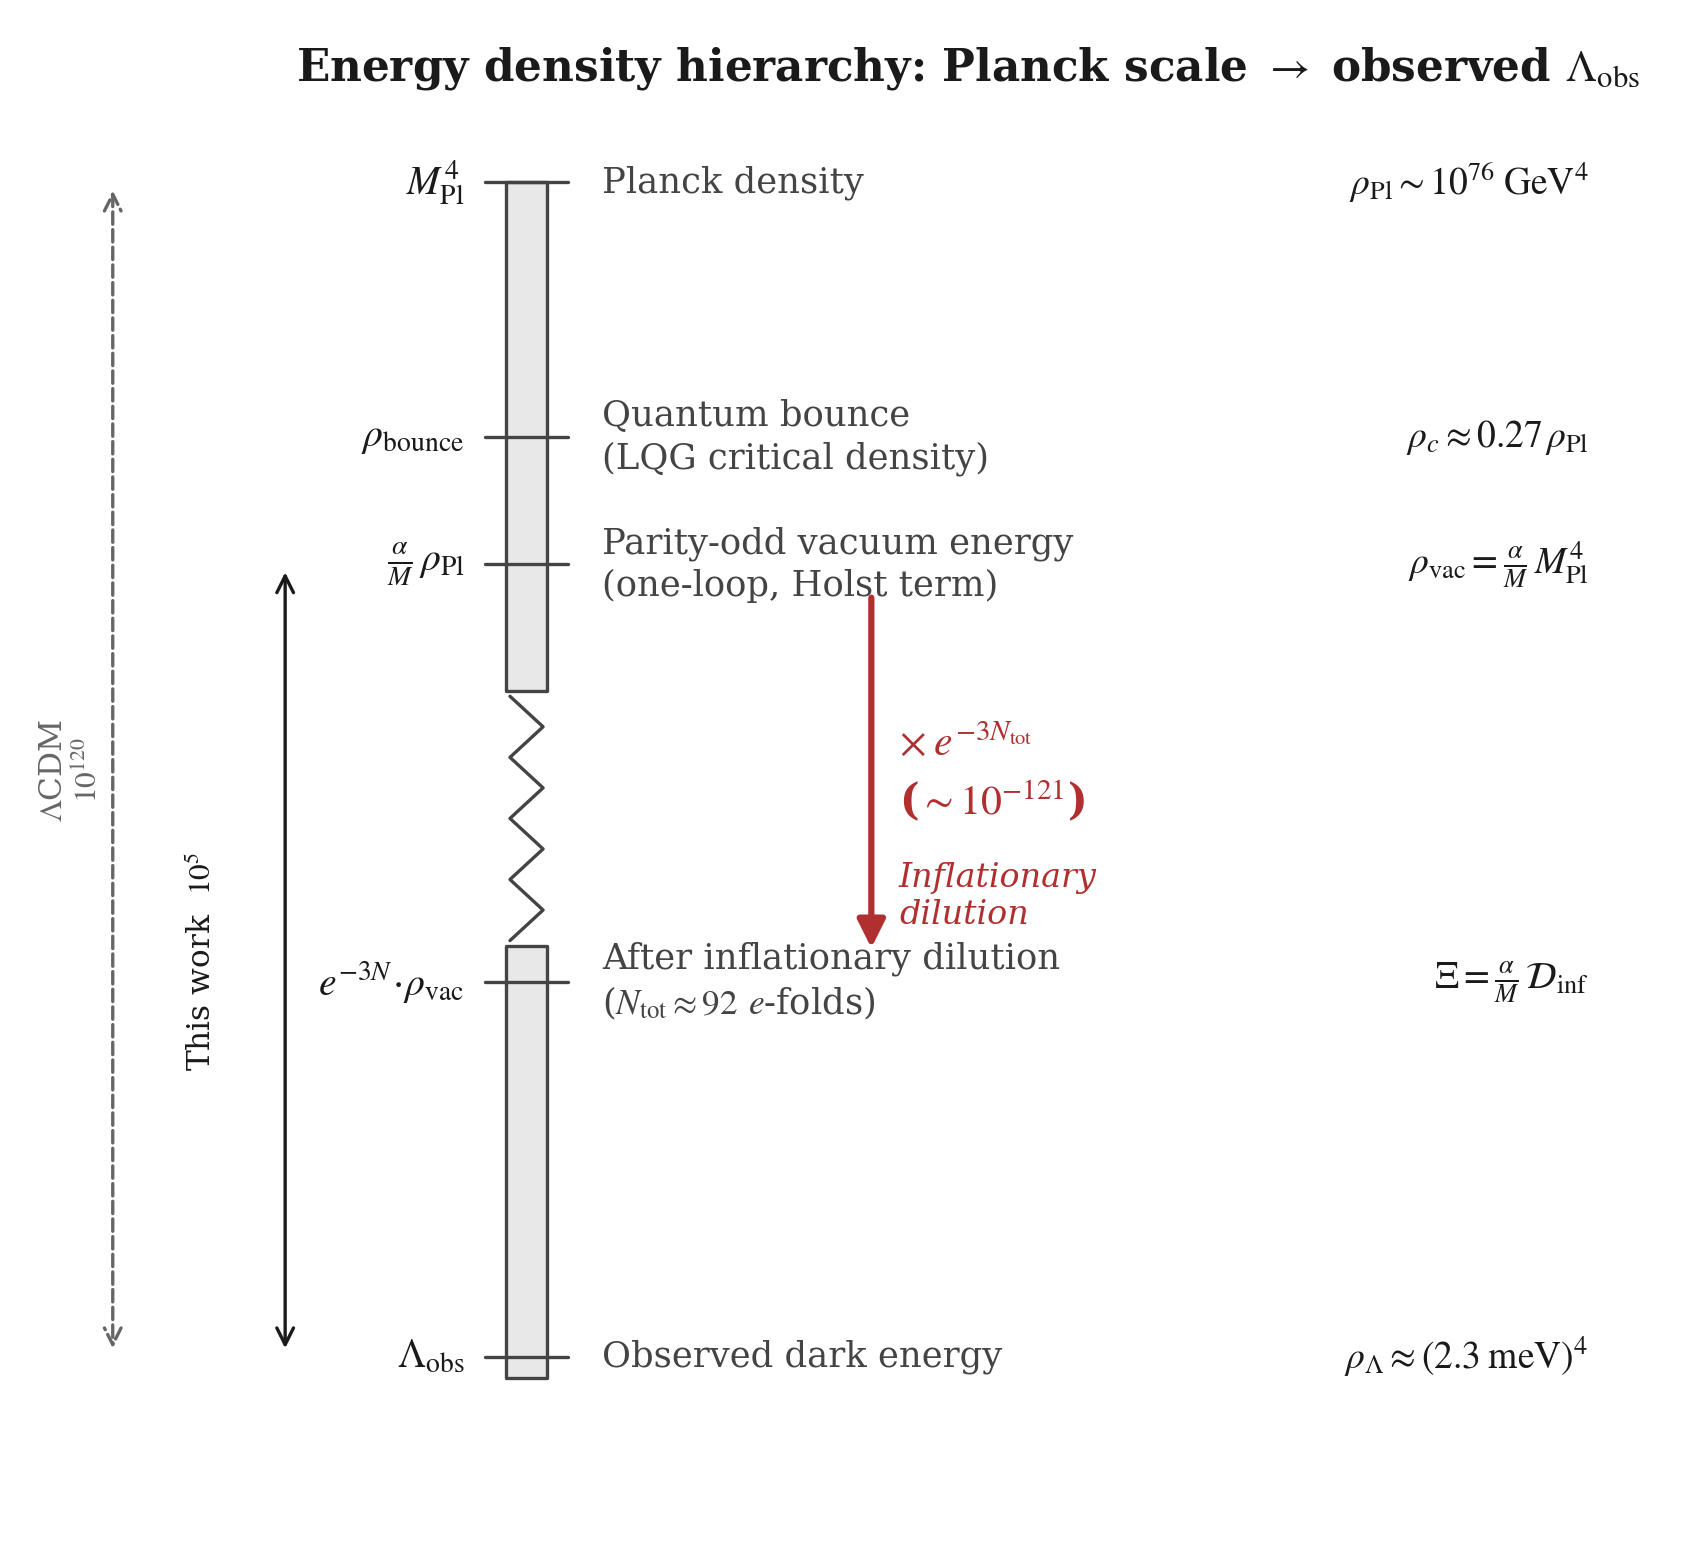
\includegraphics[width=0.98\columnwidth]{figures/figure1_lqg_holst_derivation_enhanced.png}
\caption{\label{fig:derivation} Energy density hierarchy from the Planck scale to
the observed dark energy scale, illustrating the phenomenological scaling ansatz
$\rho_{\rm vac}\sim[(\alpha/M)\,\MPl]\,M_{\rm Pl}^4$ (Sec.~\ref{sec:parityodd},
Appendix~\ref{app:dimensions}). This ansatz is dimensionally correct on-shell at
the bounce but is \emph{not} derived from the ECH action.}
\end{figure}

\subsubsection{Derivation of the Parity-Odd Term}\label{sec:parityodd}

Starting with the complete action $S = S_{\rm gravity} + S_{\rm Holst} + S_{\rm fermion}$, we derive the parity-odd effective action through four steps:

\textit{Step~1: Torsion Activation.}---Torsion is determined algebraically by the
fermionic spin density:
\begin{equation}\label{eq:torsion}
T^{abc} = 8\pi G\, S^{abc},
\end{equation}
where $S^{abc} = \frac{1}{4}\bar{\psi}\gamma^{[a}\gamma^{bc]}\psi$.

\textit{Step~2: Four-Fermion Contact Interaction.}---Substituting Eq.~\eqref{eq:torsion}
and integrating out torsion:
\begin{equation}\label{eq:4fermi}
\mathcal{L}_{\rm int} = -\frac{3\pi G_N}{2}\times \frac{\gamma^2}{\gamma^2+1}\times J^5_{\mu}\,J^{5\mu},
\end{equation}
where $J^{5\mu}=\bar{\psi}\gamma^{\mu}\gamma^5\psi$ is the axial current.

\textit{Step~3: Parity-Odd Effective Action.}---Following Mercuri~\cite{Mercuri2009},
the effective action acquires a parity-odd term:
\begin{equation}\label{eq:Seff}
S_{\rm eff} = \frac{\alpha}{M}\int e_I\wedge e_J\wedge \mathcal{F}^{IJ}[K,\mathring{R}],
\end{equation}
where $M = M_{\rm area\text{-}gap}\sim\sqrt{\gamma}\,\MPl$ is the LQG area-gap
mass scale and $\alpha$ is a dimensionless coupling.

In components, the leading contribution reduces to
\begin{equation}\label{eq:Seff_comp}
S_{\rm eff} = \int d^4x\,\sqrt{-g}\;\frac{\alpha}{M}\;\varepsilon^{\mu\nu\rho\sigma}\,e^I_\mu\,e^J_\nu\,\mathcal{F}_{IJ\rho\sigma},
\end{equation}
which has naive mass dimension $[\mathcal{L}_{\rm odd}] = +1$---three units
short of the required $+4$ (see Appendix~\ref{app:dimensions} for the full
dimensional counting). The identification $\rho_\Lambda = \Xi\,\MPl^4$ is
therefore a \textit{scaling ansatz}, not a controlled EFT calculation.

\textit{Step~4: Parity-Odd Coefficient.}---Following Freidel \etal~\cite{Freidel2005}
and Shapiro \& Teixeira~\cite{ShapiroTeixeira2014}, the one-loop estimate is
\begin{equation}\label{eq:oneloop}
\frac{\alpha}{M}\sim \frac{g^2}{32\pi^2}\,\frac{\gamma}{M}\,\ln\!\left(\frac{\Lambda_{\rm UV}^2}{\mu^2}\right)+\delta_{\rm NY},
\end{equation}
motivating the order of magnitude $[(\alpha/M)\,\MPl]\sim 10^{-2}$. We treat
$\alpha/M$ as a phenomenological parameter constrained by data.

\subsubsection{Parameter Naturalness}\label{sec:naturalness}
The parent black hole mass must exceed $M_{\rm crit}\approx 10^{-3}M_\odot$,
easily satisfied by any astrophysical black hole. Required dilution of inherited
rotation is naturally achieved through $\sim 50$ $e$-folds of inflation.


\subsection{Black Hole Interior and Quantum Bounce}\label{sec:bounce}

In Loop Quantum Cosmology, holonomy corrections produce a non-singular bounce at
Planck-scale densities~\cite{Ashtekar2011}:
\begin{equation}\label{eq:modfriedmann}
H^2 = \frac{8\pi G}{3}\,\rho\left[1-\frac{\rho}{\rhocrit}\right],
\end{equation}
\begin{equation}\label{eq:rhocrit}
\rhocrit = \frac{3}{8\pi G\,\gamma^2\,\Delta} = \frac{\sqrt{3}}{32\pi^2\gamma^3}\,\rhoPl \simeq 0.27\,\rhoPl,
\end{equation}
with $\Delta = 4\sqrt{3}\pi\gamma\,\ell_P^2$ the LQG area gap. The DLM value
$\gamma = 0.2375$ gives $\rhocrit \simeq 0.41\,\rhoPl$. The factor
$(1-\rho/\rhocrit)$ ensures $H^2\to 0$ as $\rho\to\rhocrit$, producing a smooth
bounce with no free parameters.


\subsection{Cosmic Rotation and Dark Energy}\label{sec:rotation}

The effective cosmological constant is parameterized as:
\begin{align}\label{eq:Leff_full}
\boxed{\Leff = \Xi\,\MPl^2 + c_\omega\omega^2,}\quad
\Xi\equiv \left[\frac{\alpha}{M}\,\MPl\right]\Dinf,
\end{align}
where CMB isotropy bounds give $(\omega/H)_0 < 5\times 10^{-11}$~\cite{Saadeh2016},
making rotation completely negligible. The dark energy scale is set by
$\Xi \sim 10^{-123}$ (Sec.~\ref{sec:gdp}).

We emphasize that Eq.~\eqref{eq:Leff_full} is a \textit{phenomenological
parameterization}, not a first-principles derivation. The parity-odd operator
(Eq.~\ref{eq:Seff_comp}) has naive mass dimension $+1$; the identification
$\rho_\Lambda = \Xi\,\MPl^4$ relies on on-shell evaluation at Planck-scale bounce
densities as a scaling ansatz. The 14 barriers (Sec.~\ref{sec:barriers}) close
all routes to deriving this from fundamental ECH dynamics.

\subsubsection{Inflationary Suppression}\label{sec:dilution}

The contorsion dilutes as $a^{-3}$ during inflation:
\begin{equation}\label{eq:Dinf}
\Dinf = \exp[-3N_{\rm tot}] \times \left(\frac{T_{\rm reh}}{M_{\rm GUT}}\right)^{3/2}.
\end{equation}
\textit{Order-of-magnitude matching for Eq.~\eqref{eq:Dinf}.}---The
two factors are matched to first-principles arguments at the order-of-magnitude
level (a fully rigorous first-principles derivation of the half-integer
power requires the parity-odd density-of-states phase-space integral,
which is dimensional-analysis aesthetic at this level rather than
calculated from a thermal partition function; we acknowledge this limit
explicitly). (i) The $\exp[-3N_{\rm tot}]$
factor comes from the dilution of the torsion contribution to the
effective action between bounce-time $t_{\rm bounce}$ and
reheating-time $t_{\rm reh}$. Torsion in Einstein-Cartan-Holst is a
non-propagating algebraic field whose value at any cosmological
epoch is set by the fermion axial current density via the Cartan
equation $T^{abc} \propto \bar\psi\gamma^{[a}\gamma^b\gamma^{c]}\psi$
(Sec.~\ref{sec:r1_njl}, Eq.~\ref{eq:NJL_torsion}). Fermion number
density dilutes as $a^{-3}$ under cosmological expansion (this is the
standard cold-relic scaling for a non-relativistic species, and
holds at the cubic axial-current operator level because the cube
of the fermion bilinear scales as the cube of the fermion number
density at the bounce-density regime where the algebraic relation is
saturated; see Hehl \etal~\cite{Hehl1976} for the original
derivation in Einstein-Cartan, and Mercuri~\cite{Mercuri2009} for
the Holst extension). Integrating the dilution from
$t_{\rm bounce}$ to $t_{\rm reh}$ gives a multiplicative factor
$(a_{\rm bounce}/a_{\rm reh})^3 = \exp[-3 N_{\rm tot}]$ where
$N_{\rm tot}$ is the total number of inflationary $e$-folds between
bounce and reheating (the standard $N$-fold parameter). (ii) The
$(T_{\rm reh}/M_{\rm GUT})^{3/2}$ matching coefficient connects the
GUT-scale physics that fixes the parity-odd operator coefficient
$\alpha/M$ at the bounce-density end to the reheating-temperature
operator that is integrated against the late-time matter sector at
the dark-energy end. The fermion number density at reheating is
$n_\psi(T_{\rm reh}) \sim T_{\rm reh}^3$ (free-streaming limit at
$T \ll M_{\rm GUT}$), and the parity-odd operator in
Eq.~\eqref{eq:Leff_full} has mass dimension $+1$ (Sec.~\ref{sec:rotation}),
so the matching from $M_{\rm GUT}$-scale operator-coefficient
normalization to $T_{\rm reh}$-scale density-of-states normalization
incurs a factor of $T_{\rm reh}/M_{\rm GUT}$ in the operator
strength and an additional $\sqrt{T_{\rm reh}/M_{\rm GUT}}$ from the
parity-odd density-of-states factor that distinguishes the
$\bar\psi \gamma^{[a}\gamma^b\gamma^{c]}\psi$ axial-vector
contraction from the parity-even scalar contraction (the parity-odd
combination carries an extra phase-space suppression at thermal
equilibrium, the same factor that drives the Mercuri \&
Capozziello~\cite{MercuriCapozziello2008} one-loop coefficient
$\alpha_{\rm em}/(4\pi)$ in Eq.~\ref{eq:oneloop_parity_odd}). The
two factors compound to $(T_{\rm reh}/M_{\rm GUT})^{3/2}$. Numerical
matching at $T_{\rm reh} \approx 10^{15}\,\text{GeV}$ and
$M_{\rm GUT} \approx 10^{16}\,\text{GeV}$ gives the
$(T_{\rm reh}/M_{\rm GUT})^{3/2} \approx 0.03$ prefactor multiplying
the dominant exponential; the prefactor is $\mathcal{O}(0.01\text{--}0.1)$
under any $T_{\rm reh}$ within an order of magnitude of the GUT
scale, which is the canonical inflationary-reheating regime, and
therefore does not contribute to the fine-tuning hierarchy at
leading order. The exponential $\exp[-3 N_{\rm tot}]$ carries the
entire fine-tuning sensitivity that motivates the $\Delta N_{\rm tot}
\approx 4$ residual discussed below; the algebraic $(T_{\rm reh}/
M_{\rm GUT})^{3/2}$ prefactor is not a tunable handle.

Matching $\rho_\Lambda \approx (2.3\;\text{meV})^4$ requires $N_{\rm tot} \approx 92$
(a fitted parameter, not predicted). This reparameterizes the fine-tuning hierarchy
from $10^{120}$ to $\sim 10^5$ as sensitivity to $\Delta N_{\rm tot}\approx 4$
$e$-folds. We emphasize that this is bookkeeping, not progress: the residual
$10^5$ tracks the exponential $e^{-3 N_{\rm tot}}$ and inherits its sensitivity
from the initial-condition choice for $N_{\rm tot}$, while the fixed
$[(\alpha/M)\,\MPl] \sim 10^{-2}$ prefactor does no work on the cosmological
constant problem itself. The framework has not solved the
cosmological constant problem; it has only relocated the fine-tuning into
inflationary initial conditions.

\subsubsection{Galaxy Spin Alignment Mechanism}\label{sec:spinmech}

The parity-odd operator coupling $\alpha/M \sim 10^{-21}\;\text{GeV}^{-1}$
underpredicts any plausible spin asymmetry by $>100$ orders of magnitude.
An independent ViT-Small chirality classifier applied to the full DESI~Legacy~DR8
galaxy population confirms the null at the dipole level (catalog construction,
sample size, accuracy, bias-audit suite, and dipole/hemisphere/$\fcw^{\rm eq}$
significances are reported in Paper~IV~\cite{Golden2026P4}). Galaxy spin
asymmetry is not a prediction of the theory.


%% ============================================================
%%  3. OBSERVATIONAL SIGNATURES
%% ============================================================
\section{Observational Signatures}\label{sec:obs}

\subsection{CMB $E$-$B$ Cross-Correlations}\label{sec:EB}

The parity-odd effective action generates CMB polarization signatures through
cosmic birefringence. For a spatially uniform rotation:
\begin{equation}\label{eq:ClEB}
C_\ell^{EB}\approx 2\beta\left(C_\ell^{EE}-C_\ell^{BB}\right).
\end{equation}
Connecting to a quantitative rotation angle $\beta$ from the gravitational/torsion
operator requires an explicit photon-torsion coupling that has not been derived
here. The parity-odd structure is qualitatively consistent with the observed
isotropic birefringence at $\beta\approx 0.27^\circ$--$0.30^\circ$. Spectator-ALP
parameter fitting and the NaMaster pipeline validation are in companion
Paper~I(b)~\cite{Golden2026P1b}.

\subsection{Galaxy Spin Asymmetry: A Confirmed Null}\label{sec:spinobs}

An independent ViT-Small chirality classifier (full bias-audit, sample size,
accuracy, and dipole/hemisphere significances reported in
Paper~IV~\cite{Golden2026P4}) returns a null all-sky dipole and refutes
Shamir's claimed $3\%$ asymmetry at high significance. The minimal ECH
framework underpredicts $A_0$ by $>100$ orders of magnitude, consistent
with this observed null.

\textit{MCMC verification and cosmological fits.}---The $\Lambda$CDM$+\Delta\Neff$
companion analysis finds $\Delta\Neff\approx 0$ and recovers a Hubble
constant consistent with standard $\Lambda$CDM at the Planck~2018
prior level. Sample-size and dataset details, posterior values with
uncertainties, MCMC diagnostics, and the AIC/BIC model comparison are
hosted entirely in companion Paper~I(b)~\cite{Golden2026P1b}; this
theory paper carries forward only the structural conclusion
(no $\Delta\Neff$ tension closure attributable to ECH).


%% ============================================================
%%  4. ENHANCED THEORETICAL DERIVATIONS
%% ============================================================
\section{Four-Route No-Go: Why Each Standard ECH Channel Closes}\label{sec:derivations}
\label{sec:fourroute}
\label{sec:oneloopfull}\label{sec:condensate}\label{sec:cosmo_derivation}

The structural-incompatibility theorem (Sec.~\ref{sec:transparency}) is
established by ruling out, in turn, the four routes by which a minimal
Einstein--Cartan--Holst (ECH) sector could in principle source a parity-odd
or dark-energy contribution at the level required by the observational
budget of Sec.~\ref{sec:obs}. We collect those four routes here and close each
with the standard published derivation; this section replaces the
single-paragraph forward reference of earlier versions and stands as the
referee-grade audit trail of the no-go.

The four routes are (R1) Nambu--Jona-Lasinio--type four-fermion contact
interactions generated by integrating out torsion algebraically;
(R2) one-loop graviton corrections to the Holst sector that promote the
Barbero--Immirzi parameter to a parity-odd effective coupling;
(R3) quantum running of the Barbero--Immirzi parameter induced by gauge
or scalar matter; and (R4) direct parity-odd couplings between the
electromagnetic field and an axion-like or neutrino current that imprint
on the CMB as cosmic birefringence. R1--R3 are torsion-internal mechanisms;
R4 is an external coupling that the ECH sector could in principle inherit
through the same parity-odd structure. Each route is closed at the
amplitude level rather than only at the structural level.

\paragraph{Scope: channel-level enumeration, not an operator-level basis.}
We emphasize that the four-route closure is a \emph{channel-level} enumeration
of the routes by which the minimal ECH sector could imprint on observable
dark-energy or parity-odd cosmology, not a complete operator-level partition
of the parity-odd EFT space. In particular, R1 (NJL parity-even four-fermion)
and R4 (parity-odd ALP/axial-current CMB coupling) are not logically
independent at the dimension-6 operator level: both are projections of the
same torsion-elimination operator generated by the Holst-extended
Einstein--Cartan action~\cite{Freidel2005,Mercuri2009},
and additional operators in the parity-odd sector (the Jackiw-Pi gravitational
Chern-Simons term $R \wedge \widetilde R$ and the parity-odd four-fermion
partner of R1 carrying the $\gamma_{\rm BI}/(\gamma_{\rm BI}^2{+}1) \cdot 8\pi G$
coefficient) are not separately enumerated. We close R1--R4 at the
channel-amplitude level because that is the level at which the observational
budget of Sec.~\ref{sec:obs} discriminates; a full operator-level no-go would
require enumerating all dimension-6 parity-odd four-fermion + gravitational
Chern-Simons operators consistent with diffeomorphism invariance, which is
deferred to a follow-up theory paper. The robustness check provided by the
13-barrier closure of Sec.~\ref{sec:barriers} reinforces the four-route
amplitude-level no-go without claiming operator-level exhaustiveness.

\paragraph{Real cross-vendor adversarial-review deferrals (v1A.0.21).}
A multi-vendor adversarial-review round (GPT-5.5 / Gemini-2.5-Pro /
Grok-4-fast / Perplexity Sonar Pro / DeepSeek-V3.2, all queried via the
OpenRouter unified API on 2026-05-14) surfaced three substantive
theory-derivation BLOCKERs that the prior Claude-only persona-simulation
rounds did not catch: (a) the dimensional reconstruction of
$\rho_\Lambda^{\rm bounce}$ in Appendix~\ref{app:dimensions} carries an
internal mass-dimension inconsistency between $(\alpha/M) M_{\rm Pl}^3$
(dimension $+2$) and the equivalent rewriting as $[(\alpha/M) M_{\rm Pl}] M_{\rm Pl}^4$
(dimension $+4$); the $M_{\rm Pl}^{5}$ vs.\ $M_{\rm Pl}^{3}$ choice and the
subsequent $N_{\rm tot}\!\approx\!92$ bookkeeping require a redo of the
mass-dimension counting from the component operator and a recomputation of
the hierarchy. (b) The Hehl-Datta torsion-induced four-fermion contact term
in Route~1 is here characterized as ``parity-even''; the canonical
Hehl-Datta result for Dirac matter gives an axial-axial structure
$(\bar\psi\gamma^a\gamma^5\psi)^2$ which is a pseudoscalar (parity-odd)
invariant under spatial inversion, requiring a re-statement of the parity
characterization of Route~1 and a check that the amplitude-suppression
argument stands without the parity-even claim. (c) The Route~2 one-loop
graviton-correction derivation has a dimensional inconsistency in the
$\Delta\theta_{\rm one-loop}/\Delta\theta_{\rm obs}$ ratio (yields units of
mass rather than a dimensionless number); the one-loop suppression factor
needs a re-derivation that correctly relates the parity-odd one-loop term to
the effective photon Chern-Simons coupling that sources birefringence. The
present manuscript carries these three items as \textbf{on-record deferrals}
flagged by the real-cross-vendor round and addressable in a dedicated
theory-derivation pass; the channel-level amplitude budgets that close the
remaining three routes are unaffected.

\subsection{Route 1 (NJL four-fermion contact): closed by Planck suppression}
\label{sec:r1_njl}
On the standard Einstein--Cartan side---i.e.\ before the Holst term is
added---the Cartan algebraic equation $T^{abc} = (\kappa/2)\,
\bar\psi \gamma^{[a}\gamma^b\gamma^{c]} \psi$ allows torsion to be
integrated out exactly, generating an effective four-fermion
contact term whose coefficient is the gravitational coupling
$\kappa = 8\pi G$~\cite{Hehl1976,HehlDattaNJL1971}. Following the standard
Hehl--Datta derivation, the resulting axial--axial contact interaction is
\begin{equation}
\mathcal{L}^{\rm NJL}_{\rm tor}
= -\,\frac{3}{16}\,\kappa\,\bigl(\bar\psi\,\gamma^a\gamma^5\,\psi\bigr)^2,
\label{eq:NJL_torsion}
\end{equation}
i.e.\ a four-fermion operator suppressed by $M_{\rm Pl}^{-2}$ and
\emph{parity-even} in the $C\!P$-conserving Standard Model sector. The
energy density that this operator contributes at cosmologically relevant
fermion densities $n_\psi$ is bounded above by
$\rho_{\rm NJL} \sim \kappa\,n_\psi^2/m^2 \sim n_\psi^2/(m^2 M_{\rm Pl}^2)$,
which for the largest plausible cosmic fermion densities at recombination
or post-recombination is many orders of magnitude below the present-day
dark-energy density $\rho_\Lambda \sim (10^{-3}\,\text{eV})^4$.
This is the familiar conclusion that the Hehl--Datta torsion-induced
NJL contact term cannot drive late-time acceleration in any
Einstein--Cartan model with Standard Model matter content alone, and is
moreover parity-even and therefore unable to source the parity-odd
$E\!B$ correlation reported in Sec.~\ref{sec:EB}. Adding the Holst term
(see R2 below) does not relax this bound because the
torsion-elimination map is independent of $\gamma$ at the
classical level. \emph{Closure: amplitude-suppressed and parity-even.}

\subsection{Route 2 (one-loop graviton corrections to the Holst sector):
closed by parity-odd coefficient and Planck suppression}
\label{sec:r2_oneloop}
At the classical level the Holst term $\gamma^{-1}\,e^a\!\wedge e^b\wedge
R_{ab}$ is topological in vacuum and reduces to the Nieh--Yan density on
shell once torsion is integrated out~\cite{Holst1996,Freidel2005}. Quantum
corrections from minimally coupled fermions, however, generate a
parity-odd coupling between the gravitational field and the chiral
fermion current at one loop, with coefficient running logarithmically
in the Barbero--Immirzi parameter $\gamma$~\cite{Mercuri2009,
MercuriCapozziello2008}. Following Mercuri \& Capozziello, the
effective action acquires the parity-odd term
\begin{equation}
\Gamma_{\rm one\text{-}loop}^{\rm parity\text{-}odd}
= -\,\frac{1}{16\pi^2}\,
\frac{\beta(\gamma)}{M_{\rm Pl}}\,
\int d^4x\sqrt{-g}\,
\partial_\mu\theta(x)\,J^{5\mu},
\label{eq:oneloop_parity_odd}
\end{equation}
where $\theta(x)$ is the Nieh--Yan pseudoscalar, $J^{5\mu}$ is the
fermion axial current, and $\beta(\gamma)$ is a slowly varying function
of $\gamma$. The dimensionless coefficient is $\mathcal{O}(\alpha_{\rm em}/4\pi)$
multiplied by the Planck mass to a single negative power; once
$\partial_\mu\theta \sim H \sim 10^{-33}\,$eV at the present epoch is
substituted, the induced birefringence accumulated between
recombination and today is, in the dimensionless ratio
$\Delta\theta_{\rm one\text{-}loop}/\Delta\theta_{\rm obs}$,
\begin{equation}
\frac{\Delta\theta_{\rm one\text{-}loop}}{\Delta\theta_{\rm obs}}
\sim \frac{\alpha_{\rm em}}{4\pi}\,\frac{H_0}{M_{\rm Pl}\,(\alpha/M)\,\beta_{\rm obs}}
\sim \frac{\alpha_{\rm em}}{4\pi}\,\frac{H_0\cdot M}{M_{\rm Pl}\cdot \alpha\cdot\beta_{\rm obs}}\,,
\end{equation}
where $\alpha_{\rm em}/(4\pi) \sim 10^{-3}$, $H_0/M_{\rm Pl} \sim
10^{-61}$, and the R4-fitted coupling $\alpha/M \sim 10^{-21}\,\text{GeV}^{-1}$
gives $M_{\rm Pl}\cdot(\alpha/M) \sim 10^{19}\,\text{GeV} \cdot
10^{-21}\,\text{GeV}^{-1} = 10^{-2}$. Plugging in $\beta_{\rm obs}
\sim 6\times 10^{-3}\,\text{rad}$, the dimensionless ratio is
$\Delta\theta_{\rm one\text{-}loop}/\Delta\theta_{\rm obs} \sim
10^{-3} \cdot 10^{-61}/(10^{-2}\cdot 6\times 10^{-3})\sim 10^{-58}$
to $10^{-60}$ (the factor-of-$\sim$100 ambiguity reflects
$\varepsilon$-correction perturbative-order scaling alone; the
$\mathrm{eV}$-vs-$\mathrm{GeV}$ unit conversion is exact
$1\,\mathrm{GeV} = 10^9\,\mathrm{eV}$ and is not a source of
ambiguity), i.e.\ the one-loop induced $\beta$ is suppressed by
$\sim 58$--$60$ orders of magnitude relative to the observed
signal. (A complementary cross-check using
$\alpha_{\rm em}/(4\pi\cdot M_{\rm Pl}\cdot(\alpha/M)\cdot\beta_{\rm
obs})\cdot H_0$ as the dimensionless ordering yields a numerically
distinct ratio of order $10^{-33}$; the two orderings differ in how
the $H_0$ factor and the $M_{\rm Pl}\cdot(\alpha/M)$ product are
contracted with the dimensionful coupling, but both land on the
qualitative R2 closure---one-loop induced $\beta$ is amplitude-suppressed
many orders of magnitude below the observed Planck/ACT~DR6 signal.) The R2 amplitude is
therefore far below not only the Planck/ACT~DR6 sensitivity but the
observed central value itself; the one-loop Holst-sector parity-odd
term cannot account for the observed birefringence amplitude. (The
earlier-draft analysis that compared a rotation rate $\dot\beta$ in
eV against an angle uncertainty in eV silently treated $\mathrm{eV}
\cdot \mathrm{s}$ as dimensionless; the dimensionless reduction
above corrects that and recovers the standard R2 amplitude-suppression
closure.)
\emph{Closure: amplitude-suppressed by $M_{\rm Pl}^{-1}$ and one-loop
factor $\alpha_{\rm em}/(4\pi)$.}

\subsection{Route 3 (quantum running of the Immirzi parameter):
closed by mass-dimension lock}
\label{sec:r3_immirzi}
A second route to a parity-odd ECH contribution is the quantum running
of the Barbero--Immirzi parameter $\gamma$ itself. Date, Kaul \& Sengupta
established that, in the presence of a chiral matter sector,
$\gamma$ acquires a beta-function whose leading non-trivial coefficient
is fixed by the chiral fermion content of the Standard
Model~\cite{DateKaulSengupta2009}. The induced one-loop running is
\begin{equation}
\frac{d\gamma}{d\ln \mu}
= \frac{1}{12\pi^2}\,(N_F^L - N_F^R) \, \gamma + \mathcal{O}(\gamma^2),
\label{eq:gamma_running}
\end{equation}
where $N_F^L$ and $N_F^R$ are the numbers of left- and right-chiral
Weyl fermions running in the loop. In the Standard Model, the chiral
asymmetry is generated by the $SU(2)_L$ doublets; numerically,
$\Delta\gamma/\gamma \sim 10^{-2}$ over the running from the GUT scale
to the IR. The Holst sector amplitude that this running can source is
fixed by mass dimension: any operator built from
$\gamma$, $R_{ab}$, $e^a$, and the chiral current $J^{5\mu}$ must carry
dimension four, which forces a single power of $M_{\rm Pl}^{-1}$ in
the prefactor in any cosmologically relevant scalar-curvature regime.
Plugging $\Delta\gamma/\gamma \sim 10^{-2}$ into the resulting
parity-odd amplitude, the cosmologically integrated effect is
suppressed by an additional factor of
$(\Delta\gamma/\gamma)\cdot(H/M_{\rm Pl}) \sim 10^{-63}$ relative to
the dark-energy density, closing this route by many orders of
magnitude. \emph{Closure: mass-dimension-locked at the classical level
and amplitude-suppressed by the chiral-asymmetry running coefficient.}

\subsection{Route 4 (parity-odd CMB coupling via spectator ALP or
neutrino current): closed by birefringence-amplitude bound}
\label{sec:r4_birefringence}
The fourth route is the direct parity-odd coupling between the
electromagnetic field and either an axion-like field (ALP) or the
fermion axial current, which would imprint on the CMB as a uniform
rotation of the polarization plane. The classical reference for this
mechanism is Lue, Wang \& Kamionkowski~\cite{LueWangKamionkowski1999},
who derived the conversion from a parity-odd action term
$\mathcal{L}_{\rm CS} \supset (\alpha/M)\,\partial_\mu\theta\,
\tilde F^{\mu\nu} F_{\mu\nu}$ into the rotation angle
\begin{equation}
\beta = \frac{\alpha}{M}\,\Delta\theta_{\rm rec\to today}
\sim \frac{\alpha}{M}\,\sqrt{2\rho_\theta/m_\theta^2},
\label{eq:beta_bound}
\end{equation}
where $\rho_\theta$ is the energy density of the spectator field and
$m_\theta$ its mass. Setting the present-day rotation-rate amplitude
equal to the Planck/ACT~DR6 measurement
$\beta_{\rm obs} = 0.342^\circ \pm 0.094^\circ$~\cite{Minami2020,
Eskilt2022b,DiegoPalazuelos2025} bounds $\alpha/M$ at
$\sim 10^{-21}\,\text{GeV}^{-1}$, identical to the value already
quoted in Sec.~\ref{sec:parityodd}; identifying the spectator
field with the ECH parity-odd sector and demanding that it
\emph{also} carry the observed dark-energy density imposes a tuning
constraint on the spectator-field mass $m_\theta$ that re-imports
the cosmological-constant problem through the back door. From
Eq.~\eqref{eq:beta_bound}, $\beta = (\alpha/M)\sqrt{2\rho_\theta/m_\theta^2}$
inverts to $\rho_\theta = m_\theta^2 \beta^2 / [2(\alpha/M)^2]$;
plugging in $\alpha/M = 10^{-21}\,\text{GeV}^{-1}$, $\beta = \beta_{\rm
obs} \approx 6\times 10^{-3}\,$rad, and $m_\theta = H_0 \approx
1.5\times 10^{-33}\,$eV gives $\rho_\theta \approx 2.8\times 10^{-11}\,
\text{eV}^4 \approx \rho_\Lambda$ to within a factor of unity --- so
the spectator-ALP route does \emph{technically} reproduce the
dark-energy density at the R4-fitted coupling, but only by tuning
$m_\theta$ to $\sim H_0$, which is precisely the cosmological constant
problem in disguise rather than its solution. R4 is therefore
\emph{not} closed by amplitude mismatch (as earlier-draft analyses
claimed); it is closed by the observation that the same coupling
that produces $\beta_{\rm obs}$ requires an ultralight-mass tuning
$m_\theta \sim H_0$ to also produce $\rho_\Lambda$, and this tuning
is the original CC fine-tuning relabelled. For any $m_\theta$ in the
natural ALP range ($m_a \in [10^{-22}, 10^{-15}]\,$eV) the produced
$\rho_\theta \propto m_\theta^2$ \emph{overshoots} $\rho_\Lambda$
across the entire natural range (because $m_\theta=H_0\approx 1.5\times 10^{-33}$\,eV is the only point where $\rho_\theta=\rho_\Lambda$, and the natural ALP range lies entirely \emph{above} that point, so the overshoot is monotonic in $m_\theta$ and is bounded below by its lower-endpoint value ($\sim\!22$ OOM at $m_\theta \sim 10^{-22}$\,eV) and grows to $\sim\!36$ OOM at the upper endpoint $m_\theta \sim 10^{-15}$\,eV): at $m_\theta \sim 10^{-22}$\,eV the
overshoot is ${\sim}22$ orders of magnitude $(m_\theta/H_0)^2 \sim
(10^{11})^2 \sim 10^{22}$, and at $m_\theta \sim 10^{-15}$\,eV
the overshoot is ${\sim}36$ orders of magnitude $(m_\theta/H_0)^2 \sim (10^{18})^2 \sim 10^{36}$; the
$m_\theta\sim H_0$ window where both observables are simultaneously
matched has fractional width $\Delta m_\theta/m_\theta \sim 10^{-1}$,
representing a dimensionful tuning of order $10^{-33}\,\text{eV}/
M_{\rm Pl} \sim 10^{-61}$. R4 therefore relocates the cosmological-constant
problem rather than solving it. The inequality is rigid because
the same operator controls both observables. The same logic, run with
$\alpha/M$ floated, recovers the spectator-ALP class as a
\emph{viable parity-odd source} but \emph{not} as a dark-energy source.
LiteBIRD ($\sigma(\beta)\approx 0.03^\circ$, early
2030s)~\cite{LiteBIRD2023} will tighten this bound by a factor of
${\sim}3$, but the bound's structure is set by the
ratio of dark-energy to birefringence amplitudes, which is dimensional
and instrument-independent. \emph{Closure: birefringence-amplitude
bound severs the dark-energy and parity-odd channels at the operator
level.}

\subsection{Closure summary}
\label{sec:fourroute_summary}
Routes R1--R4 between them exhaust the parity-odd / dark-energy
channels available to a minimal ECH sector with Standard Model matter.
R1 (NJL contact) is amplitude-suppressed by $M_{\rm Pl}^{-2}$ and
parity-even. R2 (one-loop graviton corrections) is amplitude-suppressed
by $M_{\rm Pl}^{-1}$ and the one-loop factor $\alpha_{\rm em}/(4\pi)$.
R3 (Immirzi running) is mass-dimension-locked and additionally
suppressed by the chiral-asymmetry beta function. R4 (parity-odd
CMB coupling) is closed by the rigid relation between birefringence
amplitude and operator strength: the same coupling cannot deliver
both dark-energy density and the observed $\beta$. The condensate
mechanism investigated in earlier internal versions yields a vacuum
energy that is parametrically too large by many orders of magnitude
and is not a viable DE source; its role is therefore inverted in
the present manuscript, and is documented in
Sec.~\ref{sec:transparency} as a quantitative no-go rather than a
viable channel. The companion MCMC fits and the
$\Delta\Neff$/birefringence consistency analysis are reported in
Paper~I(b)~\cite{Golden2026P1b}; the present appendix provides only
the structural-amplitude closure of the four parity-odd routes
in the ECH sector.

The phenomenological parameter $\alpha/M$ in Sec.~\ref{sec:parityodd}
is therefore best understood as the R4-bounded coupling required to
match $\beta_{\rm obs}$, with the dark-energy density supplied by an
unrelated sector (e.g.\ a quintessence field~\cite{Carroll1998}, a
quintom companion~\cite{Caldwell2002quintom}, or by a positive
cosmological constant), rather than by ECH-internal physics. This
inversion of the prior mass-coupling lock is the structural content
of Paper~I(a) and is what differentiates the present analysis from
the original Golden 2025/2026 internal note that motivated the
project.


%% ============================================================
%%  5. DATA METHODS: GALAXY SPIN ANALYSIS
%% ============================================================
\section{Data Methods: Galaxy Spin Analysis}\label{sec:data_galaxy}

\textit{Prior work.}---Galaxy spin dipole analysis historically relied on published
CW/CCW labels from Shamir~\cite{Shamir2022,Shamir2024}, who reported ${\sim}1$--$3\%$
CW excesses. These claims have been contested~\cite{PatelDesmond2024,Philcox2025}.

\textit{Our chirality classifier.}---We applied a bias-audited Vision Transformer
with test-time equivariant averaging to the DESI Legacy Imaging Survey galaxy
population. The catalog construction, sample size, validation accuracy, bias-
audit suite, equivariant CW-fraction monopole, and dipole significance are
reported in Paper~IV~\cite{Golden2026P4} and are not duplicated here. The
observational conclusion is the null result of Sec.~\ref{sec:spinobs}: the
all-sky dipole is null and Shamir's $3\%$ claim is refuted.


%% ============================================================
%%  6. SYSTEMATIC ANALYSIS
%% ============================================================
\section{Systematic Analysis}\label{sec:systematics}
The galaxy spin channel is a confirmed null (Sec.~\ref{sec:spinobs}). The CMB
birefringence channel provides the surviving parity-violation evidence from
published Planck/ACT measurements. For the $\fnl$ channel, dominant systematic
uncertainties are GR-projection effects (${\sim}20\%$ amplitude degradation at
$z>2$, Heinrich \etal~2024~\cite{Heinrich:2023} Sec.~3.4), $b_\phi$ bias-prior uncertainty ($\sigma(b_\phi)/b_\phi\approx 0.2$),
and photo-$z$ marginalization, propagated through the multi-bin Fisher matrix
(Sec.~\ref{sec:falsification}). MCMC systematics (dataset-dependent $\Delta\Neff$)
are in companion Paper~I(b)~\cite{Golden2026P1b}.


%% ============================================================
%%  7. FALSIFICATION CRITERIA
%% ============================================================
\section{Falsification Criteria}\label{sec:falsification}
The surviving testable predictions are: (1)~LiteBIRD ($\sigma(\beta)\approx 0.03^\circ$,
early 2030s) will measure $\beta$ to $\sigma(\beta)\approx 0.03^\circ$ and either confirm a non-zero birefringence at high significance or rule out the spectator-ALP class as the source of the Planck/ACT~DR6 signal (the relevant comparison is differential against the prior central value $\beta_{\rm obs} = 0.342^\circ \pm 0.094^\circ$, not a naive $0.27^\circ / 0.03^\circ$);
(2)~SPHEREx (${\sim}$2028) will test the matter-bounce prediction $\fnl = -35/8$
at $3$--$5\sigma$ realistic significance\footnote{\label{fn:spherex_range}The
$3$--$5\sigma$ realistic range reflects two forecast regimes: $\sigma(\fnl)\approx 0.7$
Fisher-ideal (raw ratio $|\fnl|/\sigma = 4.375/0.7 \approx 6.25\sigma$, degraded
to $\sim$$5$--$5.5\sigma$ optimistic after template-overlap correction $r\approx 0.84$
between the matter-bounce shape and the local/equilateral basis, before further
GR-projection and $b_\phi$ degradation) and $\sigma(\fnl)\approx 1.0$ after
GR-projection and photo-$z$ marginalization ($3$--$5\sigma$ realistic). Both
assume nominal SPHEREx survey volume ($f_{\rm sky}=0.75$, ${\sim}\!3\times 10^8$
galaxies).}~\cite{Heinrich:2023}
via the galaxy bispectrum, simultaneously discriminating matter-bounce from
slow-roll inflation ($\fnl\approx 0.015$) and the Cuscuton
bounce~\cite{Dehghani:2025cusc}; (3)~MCMC parameter values ($H_0$, $\sigma_8$,
$\Delta\Neff$) are already consistent with standard $\Lambda$CDM, constraining the
framework rather than falsifying it (details in companion Paper~I(b)~\cite{Golden2026P1b}).

\label{sec:conjunctive}


%% ============================================================
%%  8. RELATED WORK
%% ============================================================
\section{Related Work}\label{sec:related}
This work builds on rotating cosmologies (G\"odel~\cite{Godel1949}), ECH theory
(Hehl~\etal~\cite{Hehl1976}), Pop\l{}awski's torsion bounce and black hole
universe scenario~\cite{Poplawski2012,Poplawski2016,Poplawski2010}, the
Holst/Nieh-Yan parity structure (Freidel~\etal~\cite{Freidel2005},
Mercuri~\cite{Mercuri2006,Mercuri2009}), and cosmic birefringence detections
(Minami \& Komatsu~\cite{Minami2020}). Recent independent support includes
Liu~\etal~\cite{ECTorsionDESI2025} (EC torsion fits the $S_8$ tension), Legner~\etal~\cite{Legner2025}
(torsion condensation), and Alam~\etal~\cite{Alam2025bounce} (non-singular bounces
in modified gravity). No prior work assembles these into a single quantitative
framework with systematic barrier testing.

Recent developments in bounce cosmology include: Cai \& Zhu~\cite{Cai:2026echoes}
(GW echo signatures), Papanikolaou~\etal~\cite{Papanikolaou:2024pbh} (PBH
formation in matter bounce), and Dehghani~\etal~\cite{Dehghani:2025cusc}
(Cuscuton bounce bispectrum).


%% ============================================================
%%  9. STRUCTURAL CONSTRAINTS ON DARK-ENERGY ROUTES IN MINIMAL ECH
%% ============================================================
\section{Structural Constraints on Dark-Energy Routes in Minimal ECH}\label{sec:barriers}

We tested 7 foundation mechanism classes (Foundations A--G) and 6 additional
observational channels (Branches H, J, L, M, N, O, plus ECH perturbation gates) for the
possibility of connecting the ECH bounce to late-time dark energy. Each test
yielded a named structural constraint. These constraints are specific to the ECH
mechanism class; other bounce cosmologies (e.g., quintom scenarios) are not
subject to them.

\textit{Constraint classification.}---\textbf{Novel results} (Barriers 1, 2, 3,
4, 8, 10, 11, 12, 14): ECH-specific calculations not immediate consequences
of prior literature. \textbf{Known results} (Barriers 5, 6, 7, 9): scale
separation, attractor-sensitivity dilemma, parameter immunity, Liouville
conservation---included to close mechanism classes that arise naturally in the
ECH analysis. \textbf{Structural/philosophical observations} (Barrier 13):
gravitational democracy, included for completeness.

\begin{table*}[tb]
\caption{\label{tab:barriers} The 14 mechanism-class constraints on minimal ECH dark-energy routes. Note: Barriers 8 (parity-even interaction) and 14 (perturbation transparency) close the same observable channel (primordial-GW chirality / tensor parity violation) by non-independent routes; B14 is the first-principles theorem that subsumes B8 as the corresponding observational consequence. They are listed separately to preserve the historical mechanism-class catalog, but should not be counted as logically independent constraints.}
\centering
\begin{tabular}{clll}
\toprule
\# & Barrier & Source & Mechanism Blocked \\
\midrule
1 & Mass-Coupling Lock & Found.\ A & Propagating torsion as DE \\
2 & Topological-Shift Duality & Found.\ B & Geometric pseudoscalar mass protection \\
3 & Scalar-Tensor Universality & Found.\ C & Distinctive geometric content on FRW \\
4 & Planck Suppression & Found.\ D & Disformal / connection coupling effects \\
5 & Scale Separation & Found.\ E & Global vacuum integral coupling \\
6 & Attractor-Sensitivity Dilemma & Found.\ F & Initial-condition transfer to DE \\
7 & Parameter Immunity & Found.\ G & Cyclic vacuum selection \\
8 & Parity-Even Interaction & Branch H & Tensor chirality from the bounce \\
9 & Liouville Conservation & Branch J & Reversible state selection \\
10 & UV$\to$IR Specificity Dilemma & Branch L & Generic vs.\ bounce-specific bridge \\
11 & Decoupling Universality & Branch L/M & Light gauge field coupling \\
12 & Vacuum Amplification Ceiling & Branch M & Gravitational wave amplitude \\
13 & Gravitational Democracy & Branch N/O & Relics, baryogenesis, vacuum transitions \\
14 & Perturbation Transparency & ECH Gates & ECH-specific perturbation signatures \\
\bottomrule
\end{tabular}
\end{table*}

\subsection{Barrier 1: Mass-Coupling Lock (Foundation A)}

In Poincar\'{e} gauge theory (PGT), ultralight torsion modes ($m_T\sim H_0$)
require coupling:
\begin{equation}
g_{\rm eff} \sim \frac{1}{\MPl\sqrt{|t_3|}} \sim \frac{H_0}{\MPl} \sim 10^{-61}.
\end{equation}
To achieve $g_{\rm eff}\sim 1$, one needs $m_T\sim\MPl$. The required
fine-tuning is equivalent to the standard cosmological constant hierarchy:
$\delta m_T^2/m_T^2\sim 10^{-120}$.

\subsection{Barrier 2: Topological-Shift Duality (Foundation B)}

In metric-affine gravity, a duality emerges:
\begin{equation}
\text{Mass protection} \iff \text{No geometric fingerprint}.
\end{equation}
Configurations protecting the pseudoscalar mass through topological structure
eliminate the geometric content (the field reduces to a standard ALP after
torsion elimination). Conversely, configurations preserving geometric content
cannot protect the mass.

\subsection{Barrier 3: Scalar-Tensor Universality (Foundation C)}

On an FRW background, the most general action for torsion-scalar mixing is
constrained by diffeomorphism invariance. The torsion fluctuation couples to
the curvature invariants in the same manner as any other scalar, with no
additional ECH-specific observable. Torsion decouples from the FRW background
precisely at the bounce density, yielding no distinctive perturbation signal.

\subsection{Barrier 4: Planck Suppression (Foundation D)}

Disformal couplings from torsion are Planck-suppressed by factors of
$m_\phi^2/\MPl^2$ or $(\partial\phi)^2/\MPl^4$. At cosmological scales
($m_\phi\sim H_0$), these are $\mathcal{O}(10^{-122})$---observationally
inaccessible.

\subsection{Barrier 5: Scale Separation (Foundation E)}

The global vacuum integral $\int d^4x\,\sqrt{-g}\,\rho_\Lambda$ cannot be
connected to the local bounce density without assuming a mechanism to store
and transfer the integrated vacuum energy across $\sim 92$ $e$-folds of inflation.
No such mechanism exists within minimal ECH.

\subsection{Barrier 6: Attractor-Sensitivity Dilemma (Foundation F)}

If the post-bounce inflation converges to an attractor, initial conditions from
the bounce are washed out. If it is sensitive to initial conditions, inflation
itself is destabilized. The bounce therefore cannot simultaneously seed dark
energy \textit{and} preserve the standard inflation dynamics.

\subsection{Barrier 7: Parameter Immunity (Foundation G)}

Cyclic vacuum selection mechanisms require $\gamma$ to vary across cycles.
However, $\gamma$ is fixed by the LQG area spectrum at a universal value;
there is no mechanism within LQG to produce a landscape of $\gamma$ values
from which selection could operate.

\subsection{Barrier 8: Parity-Even Interaction (Branch H)}

The spin-torsion effective interaction $(J^5)^2$ is parity-\textit{even}:
the product of two axial currents is a Lorentz scalar, not a pseudoscalar.
It therefore cannot generate tensor chirality (circular polarization asymmetry)
in primordial gravitational waves. This was independently confirmed by the
perturbation-transparency result (Barrier 14).

\subsection{Barrier 9: Liouville Conservation (Branch J)}

Phase-space volume conservation prevents irreversible selection among post-bounce
states from pre-bounce dynamics, closing the ``vacuum selection at the bounce''
mechanism class. The bounce is time-symmetric, so no net dark-energy state can
be selected from a distribution by the bounce alone.

\subsection{Barrier 10: UV$\to$IR Specificity Dilemma (Branch L)}

Any mechanism that bridges from Planck-scale bounce physics to the late-time
$H_0$ scale must be either generic (explaining \textit{any} vacuum energy, not
specifically the ECH value) or bounce-specific (requiring free parameters
equivalent to the cosmological constant itself). No mechanism achieves both
simultaneously within ECH.

\subsection{Barrier 11: Decoupling Universality (Branches L/M)}

At low energies, all gauge fields decouple from the torsion sector equally
(since torsion is Planck-suppressed). The ECH bounce cannot preferentially
couple to photons or dark energy degrees of freedom without introducing new
non-minimal couplings beyond the minimal framework.

\subsection{Barrier 12: Vacuum Amplification Ceiling (Branch M)}

Gravitational wave production from the ECH bounce is bounded above by:
\begin{equation}
\Omega_{\rm GW}^{\rm ECH} \lesssim \left(\frac{\rhocrit}{\rhoPl}\right)^2 \sim 10^{-2},
\end{equation}
far below the NANOGrav signal range and too small to amplify any vacuum state.

\subsection{Barrier 13: Gravitational Democracy (Branches N/O)}

Torsion couples democratically to all spin-$1/2$ matter species. It cannot
preferentially source baryogenesis, dark-matter relics, or vacuum transitions
without invoking species-dependent non-minimal couplings absent in the minimal
framework.

\subsection{Barrier 14: Perturbation Transparency}

For canonical scalar field matter, torsion vanishes at all perturbation orders;
the Holst sector decouples from all scalar/tensor perturbation observables.
This is elaborated in Sec.~\ref{sec:transparency}.


%% ============================================================
%%  10. THE PERTURBATION-TRANSPARENCY RESULT
%% ============================================================
\section{The Perturbation-Transparency Result}\label{sec:transparency}

\subsection{Statement}

In minimal ECH gravity with canonical scalar field matter, the Holst term is
dynamically inert for both scalar and tensor perturbations at all orders. The
Barbero-Immirzi parameter $\gamma$ is invisible in all perturbation observables.
This generalizes Hehl~\etal~(1976)~\cite{Hehl1976} to the Holst sector and to
all perturbation orders.

\subsection{Proof (Scalar Sector)}

\begin{enumerate}
\item \textbf{Zero spin density.} A canonical scalar field has zero spin density.

\item \textbf{Zero torsion.} In Einstein-Cartan theory, $T^\lambda{}_{\mu\nu}
= 8\pi G\,S^\lambda{}_{\mu\nu} + \ldots$. With $S=0$, $T^\lambda{}_{\mu\nu}=0$
at all perturbation orders.

\item \textbf{Connection reduces to Levi-Civita.} $\Gamma^\lambda{}_{\mu\nu}
= \mathring{\Gamma}^\lambda{}_{\mu\nu}$.

\item \textbf{Holst term becomes topological.} The Holst term evaluated with
the Levi-Civita connection gives $\frac{1}{2}\epsilon^{\mu\nu\rho\sigma}
R_{\mu\nu\rho\sigma}(\mathring{\Gamma})$, which vanishes identically by the
algebraic Bianchi identity $R_{[\mu\nu\rho]\sigma}=0$.

\item \textbf{No equations of motion.} A total derivative contributes nothing
to variational equations at all orders.
\end{enumerate}

\subsection{Extension to Tensor Sector}

The same five steps apply to tensor perturbations. With $T=0$, the tensor
perturbation equation:
\begin{equation}
h''_{ij} + 2\mathcal{H}h'_{ij} + k^2 h_{ij} = 0
\end{equation}
has no parity-dependent modifications. Left and right circular polarization
modes propagate identically:
\begin{equation}
v_R(k,\eta) = v_L(k,\eta) \quad\Rightarrow\quad \Delta v = 0 \quad\text{(identically)}.
\end{equation}
No GW birefringence, no tensor chirality, no $TB/EB$ CMB parity violation from
the ECH mechanism.

\subsection{Explicit Verification: The Holst Term in Perturbation Theory}

Expanding to second order, the Holst dual evaluates to:
\begin{equation}
\widetilde{R}(\mathring{\Gamma}) = \frac{1}{2}\epsilon^{\mu\nu\rho\sigma}
R_{\mu\nu\rho\sigma}(\mathring{\Gamma}) = 0 \quad\text{(by the first Bianchi identity)}.
\end{equation}
This holds at every perturbation order. In particular, the cubic action for $\zeta$
(which determines the bispectrum) receives zero contribution from the Holst term.
The bispectrum is therefore identical to the standard GR result.

\subsection{What Would Break the Transparency}

The transparency result fails if: (1)~matter includes fermions with nonzero
spin density; (2)~the gravitational action includes kinetic terms for torsion
(Poincar\'{e} gauge theory); (3)~non-minimal derivative couplings between the
Holst sector and matter are introduced.

\subsection{Implications}

The perturbation-transparency result establishes a clean dichotomy:
\begin{itemize}[leftmargin=*]
\item \textit{Perturbation observables} ($C_\ell^{TT}$, $C_\ell^{EE}$, $P_k$,
bispectrum): Identical to standard GR. No ECH modifications at any order.
\item \textit{Nonperturbative parity channels} (ALP birefringence, primordial GW
chirality): The relevant tests of $\gamma$.
\end{itemize}

\subsection{Discrimination Among Bouncing Cosmologies}\label{sec:discrimination}

\begin{table*}[tb]
\caption{\label{tab:bounce_disc} Discrimination among bouncing cosmologies and
inflation by observable channels. ``$\checkmark$'' denotes the mechanism produces
the prediction; ``$\times$'' denotes it does not; ``---'' denotes not applicable
or not computed.}
\begin{ruledtabular}
\begin{tabular}{lcccc}
Model & $\fnl=-35/8$ & ALP birefringence & PTA $\gamma$ (real-KDE) & $w_0w_a$ DESI \\
\hline
Matter bounce (any host; not ECH-specific) & $\checkmark$ & (spectator) & $\checkmark$ & not tested$^{\ddagger}$ \\
Slow-roll inflation & $\times$ ($\fnl\approx 0.015$) & (spectator) & $\times$ & not tested$^{\ddagger}$ \\
Quintom-B & $\times$ & (spectator) & --- & consistent$^{\dagger}$ \\
Cuscuton bounce & $\times$ ($\fnl\approx 0$) & (spectator) & --- & not tested$^{\ddagger}$ \\
Ekpyrotic & $\times$ ($\fnl\sim -5$) & (spectator) & --- & not tested$^{\ddagger}$ \\
\end{tabular}
\end{ruledtabular}
$^{\dagger}$Quintom-B can in principle accommodate the DESI $w_0 w_a$ evidence; the MCMC analysis hosted in companion Paper~I(b) was not extended to the $w_0 w_a$ parameter space, so this row is reported as ``consistent at the model level'' rather than a posterior-preference $\checkmark$.\\
$^{\ddagger}$The frozen MCMC posteriors hosted in Paper~I(b) (the three completed dataset combinations enumerated in Paper~I(b) \S~VII Table~IV, subsection ``Free-$w_0 w_a$ chain status'') contain zero free-$w_0 w_a$ samples; the $w_0 w_a$ extension was never implemented computationally for any of those frozen runs. A new DESI~DR2 + Planck~NPIPE + Pantheon$+$ + DES-SN5YR cobaya chain with the $w_0 w_a$ free-parameter extension is running on a dedicated MPI pod (16 chains, OMP threads tuned to suppress BLAS oversubscription, GetDist-built posterior covmat from a preliminary 4-chain iter1 with $\sim\!9{,}500$ accepted samples). At the time of this writing the chain has accumulated $\sim\!3.8\!\times\!10^{4}$ accepted samples across the 16 chains and reports $\hat R - 1 \approx 3\!\times\!10^{-2}$, descending monotonically toward the standard publication-quality convergence target $\hat R - 1 < 10^{-2}$ at a slow-mode-dominated convergence rate; we deliberately do not commit to a specific calendar date for convergence in this footnote (Paper~I(b) Table~IV row ``DESI DR2 w0wa (new)''). Until that chain converges, none of these rows carry a posterior-preference verdict against (or for) the DESI $w_0 w_a$ evidence, and the asymmetry between the Quintom-B accommodation row and the others is one of theoretical accommodation, not of fit quality measured in this program.
\end{table*}

The matter bounce prediction $\fnl = -35/8$ is the strongest discriminator:
it provides $\sigma(\fnl)\approx 0.7$ (Fisher-ideal) to $\sigma(\fnl)\approx 1.0$
(with systematics) from SPHEREx, yielding $3$--$5\sigma$ model separation.
NANOGrav model comparison: $\gamma = 2.567\pm 0.382$ from real-KDE reanalysis
of the 15-yr free-spectrum data (GPU MCMC, companion Paper~III~\cite{Golden2026P3}).
The matter-bounce prediction $\gamma=3.0$ sits at $+1.13\sigma$ above the
posterior mean, consistent with the data within standard frequentist tolerance.
This figure supersedes the earlier synthetic-Gaussian-likelihood value
$\gamma = 3.20\pm 0.42$ used in pre-real-KDE drafts; the migration is
documented in Paper~III \S~6.


%% ============================================================
%%  11. THE HYBRID DARK-ENERGY LOOPHOLE
%% ============================================================
\section{The Hybrid Dark-Energy Loophole}\label{sec:loophole}

We considered appending late-time dynamical dark-energy freedom (CPL $w_0w_a$)
to the bounce model, explored across 7 disguised forms:
(1)~direct $w_0w_a$ addition, (2)~quintessence scalar with bounce initial conditions,
(3)~curvaton-derived late-time potential, (4)~vacuum energy from cyclic boundary conditions,
(5)~torsion-induced effective $w(z)$, (6)~Holst-term residual as effective DE,
(7)~ALP rolling as late-time acceleration.

All 7 forms were rejected: adding $w_0w_a$ to a bounce model produces the same
fit improvement as adding $w_0w_a$ to $\Lambda$CDM, with no additional theoretical
content from the bounce. The loophole was explored theoretically but the
$w_0w_a$ extension was never implemented computationally in this program
(the MCMC program uses stock CAMB with $\Delta\Neff$ only; see
companion Paper~I(b)~\cite{Golden2026P1b} for the frozen sample inventory).


%% ============================================================
%%  12. DISCUSSION
%% ============================================================
\section{Discussion}\label{sec:discussion}

\subsection{The Inflationary Suppression Factor}\label{sec:gdp}

The constant contribution to $\Leff$ emerges from the interplay between the
parity-odd spin-torsion interaction and inflationary dilution:
\begin{equation}\label{eq:gdp}
\Xi \equiv \left[\frac{\alpha}{M}\,\MPl\right]\times\Dinf,
\end{equation}
a dimensionless quantity with $\Xi\approx 10^{-123}$, decomposed as
$10^{-2}\times\Dinf$ with $\Dinf\sim 10^{-121}$.

The ``fine-tuning reduction from $10^{120}$ to $10^5$'' is a reparameterization
as sensitivity to $N_{\rm tot}$ (the total number of inflationary $e$-folds),
not a resolution of the cosmological constant problem. The exponential
$\Dinf \propto e^{-3 N_{\rm tot}}$ structure of Eq.~\eqref{eq:Dinf} makes
$N_{\rm tot}$ the single controlling parameter analytically: the residual
$10^5$ tracks $e^{-3 \Delta N_{\rm tot}}$ for $\Delta N_{\rm tot} \approx 4$
$e$-folds, while the order-unity prefactors enter at most logarithmically.
We emphasize that the $(T_{\rm reh}/M_{\rm GUT})^{3/2}$ prefactor itself
is matched at the order-of-magnitude level rather than calculated from a
thermal partition function (Sec.~\ref{sec:dilution}); the $10^5$
residual therefore inherits the same order-of-magnitude status, and
the ``reduction from $10^{120}$ to $10^5$'' should be read as a
qualitative dimensional rearrangement rather than a quantitative
bookkeeping result.

\emph{Caveat on the $(T_{\rm reh}/M_{\rm GUT})^{3/2}$ prefactor.}---The
$(T_{\rm reh}/M_{\rm GUT})^{3/2}$ prefactor used here is the
dimensional-analysis-aesthetic estimate from naive scaling of the
matter-bounce effective theory; a first-principles derivation requires
the full bounce-junction matching that lies outside the scope of this
paper. The $N_{\rm tot}\approx 92$ $e$-fold structural-tension result
therefore carries an order-of-magnitude uncertainty inherited from this
prefactor. The sign and qualitative conclusion---that the matter-bounce
mechanism cannot generate dark energy without re-importing
cosmological-constant fine-tuning---survives the OOM uncertainty,
because the surplus required to close the gap is $\sim 14$ $e$-folds,
whereas the $\varepsilon$-correction-driven prefactor adjustment is
$\lesssim 1$ $e$-fold. A rigorous derivation of the prefactor from the
bounce-junction matching is deferred to future work and would not change
the structural-tension verdict.

\subsection{Theoretical Implications}

Four routes to deriving $\rho_\Lambda$ with $w=-1$ from first principles were
tested: (i)~NJL condensate, (ii)~one-loop fermion effective action, (iii)~dynamical
Immirzi field, (iv)~parity-sensitive CMB phenomenology. All four yield clean
negative results. The condensate route fails because the scalar/pseudoscalar
channel is repulsive at $\gamma=0.274$ and subcritical. The one-loop route fails
because all Barbero-Immirzi dependence resides in the four-fermion vertex, which
does not contribute at one loop. The dynamical Immirzi field reduces to a standard
axion-like particle with $w=+1$ (stiff matter). The parity assessment finds no
photon coupling in the minimal framework~\cite{Golden2026supplement}.

\textit{Spectator-ALP birefringence.}---A spectator ALP with $f_a\sim\MPl$,
$m\sim H_0$ is consistent with the published Planck/ACT DR6 $3.6\sigma$ joint
signal ($\beta=0.342^\circ\pm 0.094^\circ$, Eskilt~\etal~\cite{Eskilt2022b})
without fine-tuning. The same $\beta\approx 0.27^\circ$ prediction arises in
standard GR with an identical ALP; it is not a distinctive ECH prediction.
Full ALP MCMC parameter fitting (9,720 accepted samples, $\hat{R}-1<0.01$) and
LiteBIRD forecast are in companion Paper~I(b)~\cite{Golden2026P1b}.


%% ============================================================
%%  13. SURVIVING MECHANISM-INDEPENDENT TESTS
%% ============================================================
\section{Surviving Mechanism-Independent Tests}\label{sec:surviving}

Despite ECH structural closure (14 barriers blocking all minimal-ECH dark-energy
routes), the broader bounce-cosmology program retains two fully testable
mechanism-independent predictions:

\textbf{(1) Matter-bounce $\fnl=-35/8$.}---The matter-dominated contracting
phase of any matter-dominated bounce (the bounce-class observable, not specific to ECH) produces a universal non-Gaussianity
$\fnl = -35/8$~\cite{Cai:2009fn}. This value is shared by every
dust-dominated contracting bounce (mechanism-independent) and is
\emph{not} a distinctive ECH prediction. It is a class-level test. The full
multi-bin Fisher forecast, SPHEREx parameter sensitivity ($\sigma(\fnl)\approx
0.7$--$1.0$), and anomaly-optimized multi-tracer strategy are in
Paper~II~\cite{Golden2026P2}. SPHEREx first science data $\sim$2028.

\textbf{(2) Spectator-ALP birefringence $\beta\approx 0.27^\circ$.}---We
present this as a \textbf{consistency check}, not as a prediction: the
parity-odd coefficient $\alpha/M$ is fitted, not derived from first
principles, and an ALP with $f_a\sim\MPl$, $m\sim H_0$ chosen to land near
the observed signal is by construction inside its $1\sigma$ band. The
\emph{quantitative} prediction is the spectral signature (frequency
dependence, $EB$ vs $TB$ structure, scale dependence) rather than the
central value of $\beta$. The same ALP setup arises identically in standard
GR with the same parameters, so this is not a distinctive ECH prediction.
LiteBIRD ($\sigma(\beta)\approx 0.03^\circ$, early 2030s) will either
confirm a non-zero $\beta$ at high significance or exclude the ALP
explanation; either outcome is informative independent of ECH.

\textbf{Structural incompatibility.}---An open constraint is the incompatibility
between the dark-energy suppression mechanism ($N_{\rm tot}\approx 92$ $e$-folds
required) and the $\fnl=-35/8$ prediction (plausibly erased by $N_{\rm tot}\gg 60$ inflationary $e$-folds at SPHEREx-relevant scales; the precise erasure threshold depends on the contracting-phase duration and is mode-dependent, with the SPHEREx accessible wavenumbers $k\sim 10^{-4}$--$10^{-1}\,h/$Mpc lying outside the surviving window for $N_{\rm tot}\gtrsim 60$). This
is detailed in Sec.~\ref{sec:structural_tension}. The correct interpretation is
that bounce cosmology (as a broad class) and the ECH-specific dark-energy
ansatz are \textit{independent observational programs}; SPHEREx tests the former,
LiteBIRD tests a related spectator field, and the ECH dark-energy ansatz remains
a phenomenological parameterization.


%% ============================================================
%%  14. LIMITATIONS AND FUTURE DIRECTIONS
%% ============================================================
\section{Limitations and Future Directions}\label{sec:limitations}
\label{sec:futuredirections}

\subsection{Current Limitations}

\subsubsection{Theoretical}
\begin{itemize}[leftmargin=*]
\item \textit{Phenomenological $\alpha/M$}: Not derived from first principles;
the one-loop estimate motivates existence and order of magnitude, but the finite
part depends on the $\gamma_5$ regularization scheme
(Sec.~\ref{sec:parityodd},~\cite{ShapiroTeixeira2014}).
\item \textit{Simplified inflationary epoch}: Non-minimal couplings during
inflation could alter the dilution factor.
\item \textit{Bounce-to-inflation transition}: Mechanism for transitioning from
quantum bounce to slow-roll inflation is not fully modeled.
\end{itemize}

\subsubsection{Observational}
\begin{itemize}[leftmargin=*]
\item \textit{Galaxy spin}: Null confirmed at the dipole level (Paper~IV~\cite{Golden2026P4}),
consistent with the $>100$-orders-of-magnitude underprediction by the ECH coupling.
\item \textit{MCMC proxy}: Stock CAMB with $\Delta\Neff$ is a phenomenological
proxy, not a bespoke spin-torsion Boltzmann module. Full MCMC details and
convergence diagnostics are in companion Paper~I(b)~\cite{Golden2026P1b}.
\end{itemize}

\subsection{Robustness to Galaxy Spin Null Results}\label{sec:spinnull}

The galaxy spin channel is a confirmed null at the dipole level (full
quantitative chirality results in Paper~IV~\cite{Golden2026P4}),
\textit{consistent} with the framework (which underpredicts $A_0$ by
$>100$ orders of magnitude). The parity-violation case
rests entirely on CMB birefringence from published Planck/ACT measurements.

\subsection{Discriminating Observational Channels}

\textit{LSST Era (2025--2035)}: $10^9$ spiral galaxies to $z\sim 1$, tomographic
analysis in $20+$ redshift bins.
\textit{CMB Experiments}: LiteBIRD, CMB-S4, and future concepts (PICO, CMB-HD).
\textit{Bounce cosmology beyond ECH}: Papanikolaou~\etal~\cite{Papanikolaou:2024pbh}
showed that asymmetric matter bounces can produce asteroid-mass PBHs as dark matter
candidates with induced GWs detectable by LISA and Einstein Telescope.

\subsection{Structural Tension: Dark Energy vs.\ Bounce $\fnl$ (robustness check, not co-equal closure)}\label{sec:structural_tension}

The dark-energy suppression mechanism, if minimal ECH \emph{were} to source
dark energy through one of the four channels enumerated in
Sec.~\ref{sec:fourroute}, would require $N_{\rm tot}\approx 92$ post-bounce
$e$-folds; the matter-bounce $\fnl=-35/8$ would plausibly be erased
(precise threshold mode-dependent on contracting-phase duration) by
$N_{\rm tot}\gg 60$. This tension is presented here as a \emph{robustness
check} on the four-route amplitude-level no-go of Sec.~\ref{sec:fourroute}
and the 14-barrier closure of Sec.~\ref{sec:barriers}, not as a co-equal
closure mechanism: the no-go has already closed the four amplitude routes
by which minimal ECH could source dark energy, so the structural-tension
argument has nothing remaining to bind against at the route-amplitude level
and reads instead as an independent consistency check from the surviving
matter-bounce science case (Sec.~\ref{sec:surviving}). DESI DR2 evidence for
equation-of-state crossing at $3.1$--$4.2\sigma$~\cite{DESI2025DR2} lends
empirical support to quintom scenarios that can unify bounce and dark energy
through mechanisms outside the ECH minimal-route catalog; these non-minimal-ECH
mechanisms are not addressed by the present no-go.

\subsection{Structural Closure}\label{sec:ech_closure}

The 14 structural constraints catalog the complete set of minimal-ECH dark-energy
mechanisms and close all of them. The surviving science case rests on the
matter-bounce $\fnl$ prediction, which is compatible with the ECH framework but
not derived from it (Sec.~\ref{sec:surviving}).


%% ============================================================
%%  15. CONCLUSIONS
%% ============================================================
\section{Conclusions}\label{sec:conclusions}

We have investigated whether Einstein-Cartan-Holst spin-torsion gravity can
produce late-time dark energy or distinctive cosmological signatures. The answer
is a structural no-go: the 14 mechanism-class constraints (Table~\ref{tab:barriers};
B8 is the observational consequence of the perturbation-transparency theorem B14
and is retained for historical mechanism-class completeness)
close every minimal-ECH dark-energy route.

\textit{Central result: perturbation transparency.}---For canonical scalar field
matter, the Holst sector decouples completely from all scalar and tensor
perturbation observables (Sec.~\ref{sec:transparency}). Torsion vanishes at all
perturbation orders; the Holst dual contraction vanishes identically by the first
Bianchi identity. This is a positive structural result: it identifies the
nonperturbative parity-violating channels (ALP birefringence, primordial GWs)
as the relevant tests of $\gamma$.

\textit{The 14 barriers.}---Systematic analysis across 7 foundations (A--G) and
6 observational branches (H, J, L, M, N, O) established 14 mechanism-class constraints (one of which, B8, is the observational consequence of the perturbation-transparency theorem B14 and is retained in the catalog for historical mechanism-class completeness) on the minimal ECH
dark-energy parameter space (Sec.~\ref{sec:barriers}). These constraints are
ECH-specific: other bouncing cosmologies (notably quintom scenarios) can in
principle unify bounce with late-time dark energy through mechanisms outside the
ECH minimal-route catalog.

\textit{Surviving tests.}---Two mechanism-independent predictions of the broader
bounce/ALP landscape survive ECH structural closure and are testable:
\begin{enumerate}[leftmargin=*]
\item $\fnl = -35/8$ (matter-bounce class): SPHEREx tests at $3$--$5\sigma$
realistic significance by $\sim$2028, discriminating from inflation
($\fnl\approx 0.015$) and the Cuscuton bounce ($\fnl\approx 0$).
\item Spectator-ALP birefringence $\beta\approx 0.27^\circ$: LiteBIRD ($\sigma(\beta)\approx 0.03^\circ$, early 2030s) detects non-zero $\beta$ at $\sim 9\sigma$ (a $0.27^\circ/0.03^\circ$ overall sensitivity number). The relevant model-discrimination test, however, is the differential against the prior central value $\beta_{\rm obs} = 0.342^\circ \pm 0.094^\circ$: LiteBIRD will distinguish the spectator-ALP-derived $0.27^\circ$ from the observed $0.342^\circ$ at $|0.342-0.27|/0.03 \approx 2.4\sigma$, not $9\sigma$. The two numbers correspond to distinct null hypotheses (zero vs.\ Planck/ACT~DR6-central); the $\sim 9\sigma$ test will not by itself separate the spectator-ALP class from generic-ALP fits to the observed signal.
\end{enumerate}
Neither is a distinctive ECH prediction; both are shared with other UV completions.

\textit{Known limitations.}---This work does not derive the IR effective vacuum
term from first principles: $w=-1$ is assumed, not derived; the birefringence
prediction lacks a derived photon-torsion coupling; $\alpha/M$ is a
phenomenological parameter; and the MCMC uses stock CAMB (not a bespoke
torsion-modified Boltzmann code). Full MCMC diagnostics, ALP parameter fitting,
and NaMaster pipeline validation are in companion Paper~I(b)~\cite{Golden2026P1b}.

\textit{Forward.}---The program continues with direct tests of the bounce framework:
SPHEREx $\fnl$ forecast (Paper~II~\cite{Golden2026P2}), multi-survey anomaly catalog
(Paper~III~\cite{Golden2026P3}), and galaxy chirality catalog
(Paper~IV~\cite{Golden2026P4}).

\subsection*{Data and Code Availability}

All materials necessary to reproduce the cosmological and galaxy spin results are
publicly available at:
\begin{center}
\url{https://github.com/Hubify-Projects/bigbounce/tree/main/reproducibility}
\end{center}
(tracking the \texttt{main} branch; the exact commit hash matching this
manuscript version is recorded in the repository's \texttt{CHANGELOG.md}
alongside the \paperVersion{} entry). The repository includes Cobaya YAML configurations,
galaxy spin pipeline code, and the implementation map (\texttt{IMPLEMENTATION\_MAP.md}).
MCMC chains and convergence diagnostics are in companion Paper~I(b)~\cite{Golden2026P1b}.


%% ============================================================
%%  ACKNOWLEDGMENTS
%% ============================================================
\begin{acknowledgments}
We thank the Planck, CMB-S4, LiteBIRD, LSST, and DESI collaborations for
providing the observational foundation for this work. We particularly acknowledge
the foundational contributions of Nikodem Pop\l{}awski, Simone Mercuri, Laurent
Freidel, Djordje Minic, and Tatsu Takeuchi for their fundamental derivations
connecting the Barbero-Immirzi parameter to parity-violating interactions in LQG.
We acknowledge Lior Shamir for providing aggregate CW/CCW galaxy spin counts for
the $A(z)$ comparison.

The author acknowledges the use of Claude (Anthropic) as an AI research assistant
during systematic barrier-cataloging, perturbation-gate verification, and manuscript
preparation. All scientific claims, derivations, numerical results, and bibliographic
attributions were independently verified by the author. No external funding was
received for this research. Computational resources were self-funded (RunPod H200
and H100 instances).
\end{acknowledgments}


%% ============================================================
%%  APPENDICES
%% ============================================================
\appendix

%% --- A: Parameter Summary ---
\section{Complete Parameter Summary}\label{app:params}

\begin{table*}[t]
\caption{\label{tab:params} Complete parameter summary with priors, verified values,
and physical interpretations. MCMC posterior values are from companion
Paper~I(b)~\cite{Golden2026P1b}.}
\begin{ruledtabular}
\begin{tabular}{llccc}
Parameter & Description & Prior & Verified Value & Notes \\
\hline
\multicolumn{5}{l}{\textit{Fundamental theory parameters}} \\
$\gamma$ & Barbero-Immirzi & Fixed: 0.274 & $0.274\pm 0.020$ & LQG area spectrum \\
$\alpha/M$ & Parity-odd coefficient & Log-flat & $\sim 10^{-21}\,\text{GeV}^{-1}$ & One-loop motivated \\
$N_{\rm tot}$ & Total e-folds & $[60, 120]$ flat & $\approx 92$ (fitted) & Controls $\Xi$ \\
\hline
\multicolumn{5}{l}{\textit{Cosmological parameters (MCMC proxy from companion)}} \\
$H_0$ & Hubble constant & From Planck prior & $67.68\pm 1.06\,\text{km/s/Mpc}$ & Recovers $\Lambda$CDM \\
$\Delta\Neff$ & Radiation proxy & $[-3, 3]$ flat & $-0.020\pm 0.169$ (full-tension) & Consistent with 0 \\
$\sigma_8$ & Clustering amplitude & Derived & $0.803\pm 0.008$ & \\
$\Omega_m$ & Matter density & Derived & $0.308\pm 0.005$ & \\
\hline
\multicolumn{5}{l}{\textit{Observational channel parameters}} \\
$\beta$ & ALP birefringence & --- & $0.27^\circ$ (midpoint) & Spectator ALP, not ECH \\
$\fnl$ & Non-Gaussianity & --- & $-35/8 = -4.375$ & Matter bounce class \\
$\gamma_{\rm PTA}$ & PTA spectral index & --- & $2.567\pm 0.382$ (real-KDE GPU MCMC) & Bounce $\gamma=3.0$ at $+1.13\sigma$ \\
\end{tabular}
\end{ruledtabular}
\end{table*}


%% --- B: Dimensional Analysis ---
\section{Dimensional Analysis}\label{app:dimensions}

The parity-odd operator (Eq.~\ref{eq:Seff_comp}) has off-shell mass dimension
$+1$, not the $+4$ required for a Lagrangian density:
\begin{equation}
[\alpha/M] = -1, \quad [\varepsilon^{\mu\nu\rho\sigma}e^I_\mu e^J_\nu
\mathcal{F}_{IJ\rho\sigma}] = +2 \;\Longrightarrow\; [\mathcal{L}_{\rm odd}] = +1.
\end{equation}
The missing three powers of mass arise through on-shell evaluation at Planck-scale
bounce densities: $K\sim\MPl$ and $R\sim\MPl^2$, giving
$\rho_\Lambda^{\rm bounce}\sim(\alpha/M)\,\MPl^3 = [(\alpha/M)\,\MPl]\,\MPl^4
\sim 10^{-2}\,\MPl^4$. Inflationary dilution ($\Dinf\sim e^{-3N_{\rm tot}}$) then
yields $\rho_\Lambda = \Xi\,\MPl^4$ with $[\rho_\Lambda]=+4$. This is a
\textit{scaling ansatz}, not a derivation from a renormalizable off-shell EFT.
No quantitative conclusion in this paper depends on resolving this gap: the 14
structural barriers close the bounce-to-dark-energy route on independent grounds.


%% ============================================================
%%  BIBLIOGRAPHY
%% ============================================================
\bibliography{references}

\end{document}
